% teleconnections chapter

\Chapter{pyleogrid}{An Ensemble method for Gridding Paleo Proxy Climates}

\label{chp:gridding}

\begin{refsection}

%----------------------------------------------------------------------------------------
%	SECTION 1
%----------------------------------------------------------------------------------------

\section{Introduction}  \label{sec:gridding-intro}

\todo[inline]{Write gridding introduction}

\begin{itemize}
	\item Why gridding
	\begin{itemize}
		\item Data-Model-Intercomparisons)
		\item Easier to handle
		\item Energy balance, compatibility with models, grid cell (Area) averages
		\item Stability of observation network through time
		\item Not just spatial grid, also regular timestep (problems with pseudo gridding, including time ‘windows’ or ‘slices’
		\item Understanding past climates, different forcings – independent of models (difficult from point-cloud)
		\item Filling the gaps
		\item Spatial scales (Samarthein chironomids etc)
	\end{itemize}
	\item Importance of uncertainties
	\begin{itemize}
		\item Necessary for data comparisons, interpretation skill of the data
		\item Proxy climate reconstruction uncertainties are higher (inverse modelling, not always properly defined (MAT)) than for instrumental data
		\item Age uncertainties can be high (centennial to multi-millennial)
	\end{itemize}
	\item Why Tps (can also use something else, but has been used before)
	\begin{itemize}
		\item Extrapolation to the gaps (Previous work by mauri et al and davis)
		\item Pseudo-gridding (marcott, Marsicek 2018, Margo, 2009, Bartlein et al ?2013) has holes
		\item Data assimiliation (pages2k? Need to look the paper up again) – depends on model
		\item Bayesian data assimiliation (Weitzel 2019) – depends on model
		\item Does not require interpolation of time (Marsicek 2018)
	\end{itemize}
	\item Other
	\item Introducing constraints; climate, training set size, spatial coverage etc
\end{itemize}

\section{Data}  \label{sec:gridding-data}

The ensemble based gridding method is adapted to paleo-climates. In this study, we describe the method using a large set of western Eurasian fossil pollen assemblages that have been transformed to \gls{jja} temperatures. We focus on pollen data because it is the spatially most widely available proxy during the Holocene, but it is important to mention that the reconstruction method is agnostic to the climate proxy, because it does not explicitly use the pollen assemblages but rather alters the standard climate reconstruction method under the aspect of it's methodological uncertainties. As such, the following sections describe the fossil and modern pollen database for this use case (section \ref{sec:gridding-polnet}) and the associated uncertainties of the temperature reconstruction method (section \ref{sec:gridding-mat}) and the dating of the fossil pollen samples (section \ref{sec:gridding-ageunc}).

\subsection{Pollen database}  \label{sec:gridding-polnet}

\begin{figure}
	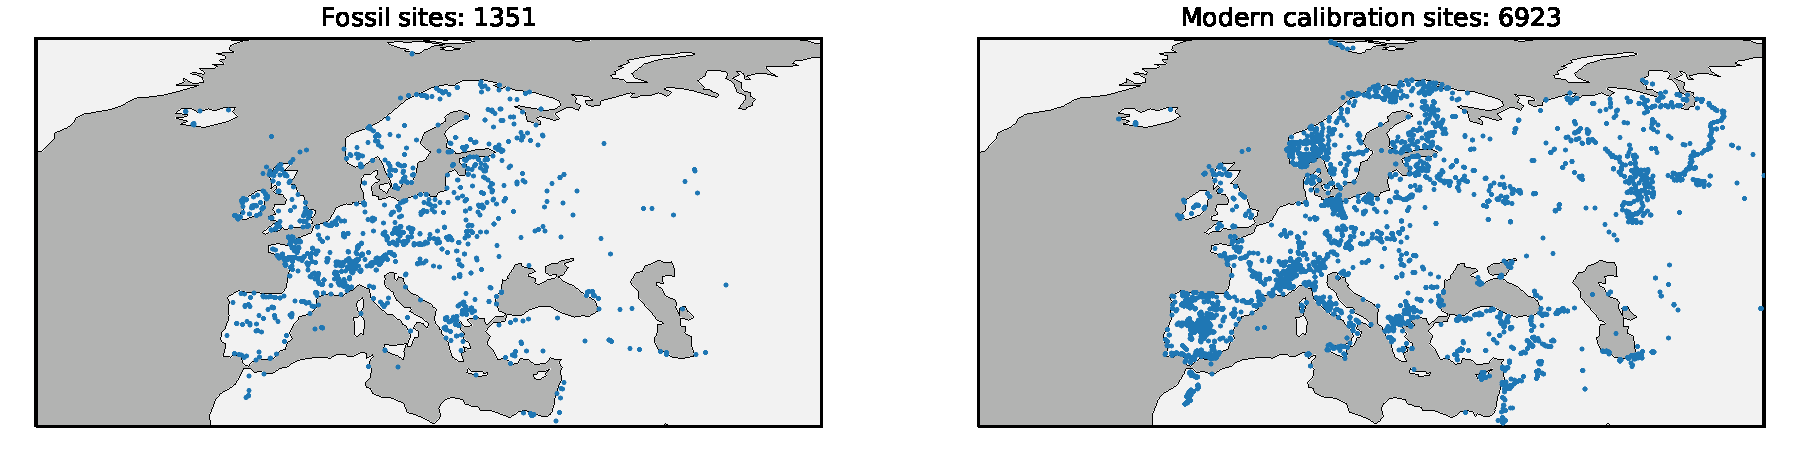
\includegraphics[width=\linewidth]{gridding-figures/sitelocs.pdf}
	\caption[Pollen Database]{Site locations of the (left) fossil and (right) modern pollen database.}
	\label{fig:gridding-fossil}
\end{figure}

The source data for this study is a subset of the latest development version of the POLNET database, a northern hemispheric, sub-tropical collection of pollen assemblages \citep{DavisKaplan2017, SommerDavisChevalierEtAl2019}. The purpose of this database is to generate the source for large-scale climate reconstruction during the Holocene (past 12'000 years) that can be used for model-data comparisons. The subset that we use in this study to describe and develop the gridding method contains fossil and modern pollen assemblages of western Eurasia, a region that has already been under investigation in the previous study by \cite{MauriDavisCollinsEtAl2015}. 

The fossil database contains raw pollen counts with in total about 1350 datasets that consists of 80500 fossil samples. The majority of the fossil pollen data (left part of figure \ref{fig:gridding-fossil}) comes from the \gls{epd} \citep[ca. 94\%]{FyfeBeaulieuBinneyEtAl2009} and other publicly available databases. The presented dataset extends the database used by \cite{MauriDavisCollinsEtAl2015} especially with a few sites towards the eastern part of the map.

The modern calibration dataset (6900 sames, see right map in figure \ref{fig:gridding-fossil}) is mainly based on the version 2 of the \gls{empd} \citep[ca. 87\%, see also chapter \ref{chp:empd}]{DavisZanonCollinsEtAl2013} and core tops of EPD (10\%) that were younger than 250 years cal BP.


\subsection{Sample site: Tigalmamine} \label{sec:gridding-sample-site}

\begin{figure}
	\captionsetup{width=1.2\linewidth}
	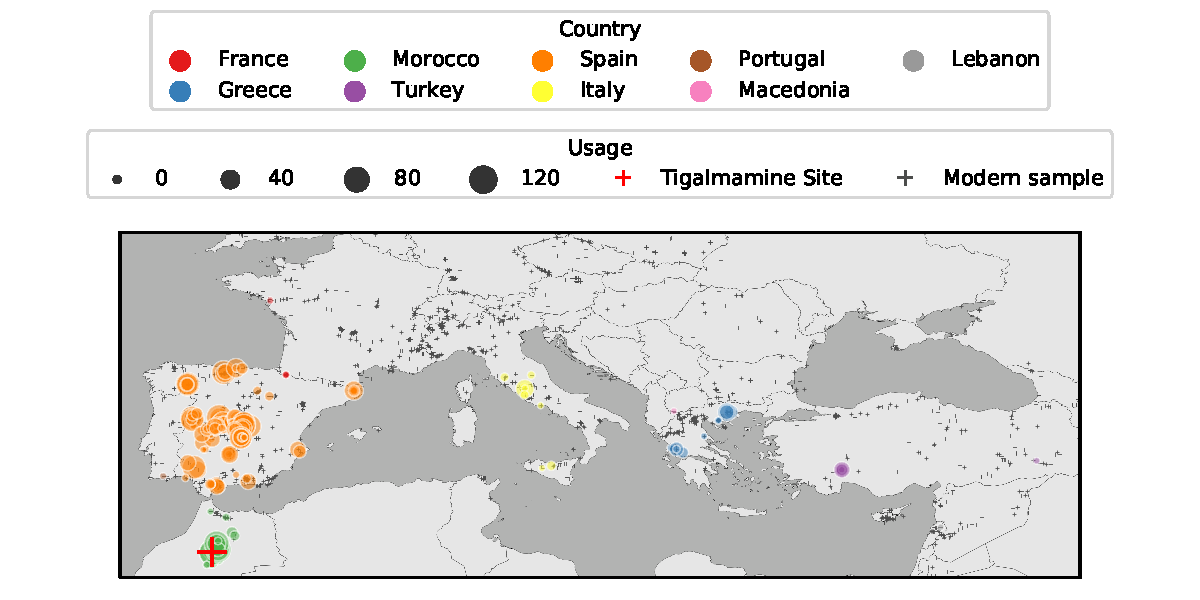
\includegraphics[width=\linewidth]{gridding-figures/tigalmamine-analogue-map.pdf} \\
	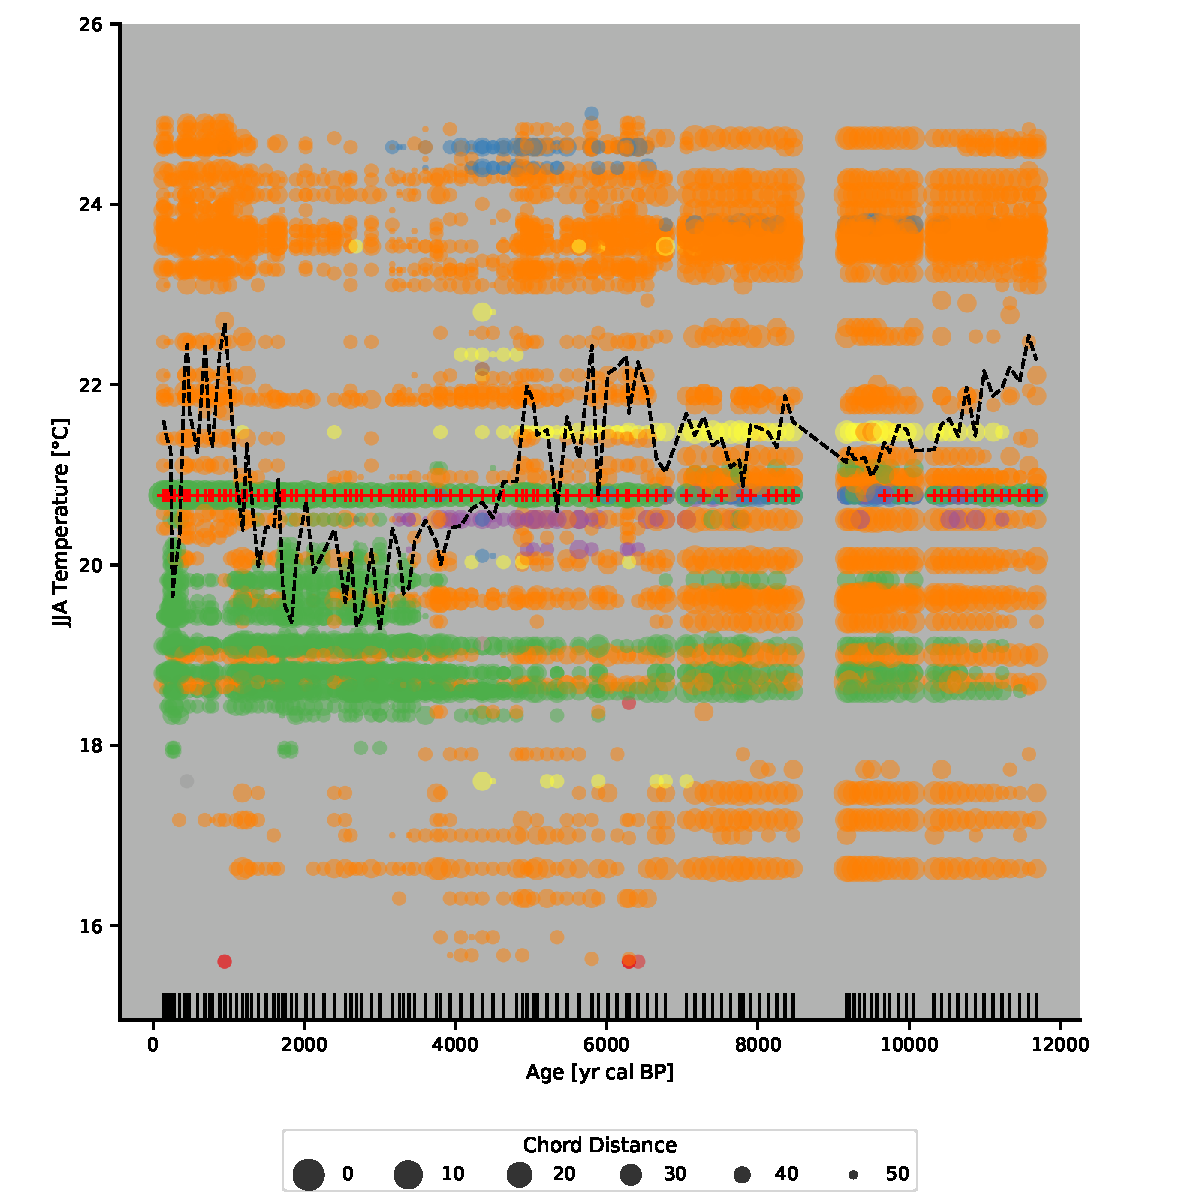
\includegraphics[width=\linewidth]{gridding-figures/tigalmamine-analogue-climates.pdf}
	\caption[Climate analogues of the Tigalmamine site]{Climate analogues of the Tigalmamine site (red cross). Every circle corresponds to one modern analogue that was one of the fifties closest analogues in at least one sample within the Tigalmamine dataset. The color-coding of each circle is based it's corresponding country (see legend at the top). The marker size in the top plot depends on the usage of the sample as modern analogue. The larger the marker, the more samples in the Tigalmamine dataset use it as modern analogue. Tiny crosses in the map show the locations of the rest of the modern calibration data. The lower plot shows the summer temperature for the analogue (y-axis) at the age of the Tigalmamine sample (x-axis). The marker size in this plot corresponds to the chord distance between modern and fossil pollen assemblage. I.e., the larger the dot, the closer (and more important) the analogue. The dashed line shows the weighted average of all the climate analogues per sample. The age of each Tigalmamine sample is shown with the vertical lines at the bottom of the plot. Red crosses in the lower plot show the Tigalmamine core top sample that has been used as an analogue in 58 out of the 110 samples.}
	\label{fig:gridding-site-analogues}
\end{figure}

We chose the pollen record of Tigalmamine in Morocco (32.9N, 5.34W, 1626m) to evaluate our method. The site was first studied by \cite{LambKaars1995}, and the pollen data was downloaded from the European Pollen Database. The chronology and choice of control points used here is that from Giesecke et al \citep{GieseckeDavisBrewerEtAl2013}. The site is well dated with 11 radiocarbon dates, and spans the entire Holocene with 110 samples. The data has been used for a previously published pollen reconstruction based on the modern analogue method \citep{CheddadiLambGuiotEtAl1998}, although this study used a calibration dataset that included modern pollen samples from Morocco that have subsequently been found to have geolocation errors \citep{DavisZanonCollinsEtAl2013}. None of these problematic modern samples have been used in our analysis. 

The site (red cross in figure \ref{fig:gridding-site-analogues}) is located on the southern edge of our study region in an area with a montane Mediterranean vegetation and climate. The Mediterranean has traditionally been considered to be a particularly challenging environment for pollen-based reconstructions because of the effects of long term human impact, and the interplay of precipitation and temperature on vegetation distribution. The fossil pollen record of Tigalmamine shows a mainly forested montane Mediterranean assemblage throughout the Holocene, dominated by evergreen oak, but with an important transition between the early Holocene and late Holocene marked by a change from deciduous Oak to Cedrus (see the pollen diagram in \cite{CheddadiLambGuiotEtAl1998}). The occurrence of Cedrus represents an interesting challenge for any pollen climate transfer function, since this particular taxa is limited in its distribution (and in our calibration dataset) to Morocco and the Lebanon region, while all of the other taxa in the assemblage are widely distributed across the Mediterranean. The strong presence of evergreen Oak also makes the site interesting, because although this taxa is mainly associated with the Mediterranean region, its distribution extends all the way up the west coast of France to Brittany.

Figure \ref{fig:gridding-site-analogues} illustrates these challenges for the particular site. The climate analogues (see next section \ref{sec:gridding-mat}) span a large summer temperature regime of about 10 degrees, from 15 to 25 °C. The upper temperature range is dominated by analogue climates from Spain (orange) which in general shows the highest number analogue matches. The early Holocene (12k to 8k BP) is dominated by modern samples from Spain, with a wider and more uniform temperature regime, when compared to the later periods. During the transition in the mid-Holocene (8k to 4k BP), analogues from across the Mediterranean Sea play a more important role, in particular from Greece, Italy and Turkey. The lower temperature regime is then dominated by Moroccan samples (green) that are of particular importance during the late Holocene (4k BP to present) due to the above mentioned presence of Cedrus. 

The weighted average of the analogues (black dashed line in figure \ref{fig:gridding-site-analogues}) is in general about one to two degrees lower than the one in \cite{CheddadiLambGuiotEtAl1998} (very likely due to the above-mentioned erroneous calibration data they used). The trends are however similar: Higher temperatures in early Holocene  (the \textit{spanish analogues} dominate) with a drop around 6k BP (Moroccan climates). Our weighted average however also shows a clear increase during the past 2000 years, again driven by spanish analogues.

The climatic and geographic space that is covered by the analogues is further discussed in section \ref{sec:gridding-temperature-sampling}.

\subsection{Site-based holocene temperature estimates}  \label{sec:gridding-mat}
A standard approach for site-based climate reconstruction from fossil pollen assemblages is the \glsfirst{mat} (also called $k$-nearest neighbors). This technique estimates the climate of the fossil sample as the (weighted) climate average of the most similar modern samples (i.e. the closest modern analogues). It has the major advantage that it requires little parameterization efforts and can be applied over a large spatial area that covers many different climate regimes \citep{MauriDavisCollinsEtAl2015}. 

For this purpose, we follow the standard approach and assign a \gls{jja} temperature values to each modern calibration sample (figure \ref{fig:gridding-modern}), taken from the corresponding grid cell in the WorldClim dataset, version 2 at 30 seconds \citep{FickHijmans2017}.

Every pollen assemblage is then transformed from raw counts to percentages, based on the total sum of terrestrial pollen counts per sample that we deem useful for the reconstruction. This excludes low samples with low counts and taxa with low occurrences. We use squared-chord distance from the R package \textit{rioja} \citep{Juggins2017} as a measure of similarity. For a given transformed fossil pollen assemblage $\left\lbrace f_{t}\right\rbrace$ and a modern pollen assemblage $\left\lbrace m_{t}\right\rbrace$, where $t=\left\lbrace1,\ldots,N\right\rbrace$ denotes one of the $N$ individual taxa in the assemblages, this distance measure is defined as

\begin{equation*}
d = \sum_{t=1,\ldots,N}\left(\sqrt{f_{t}} - \sqrt{m_{t}}\right)^2
\end{equation*}

This distance is calculated between every modern and every fossil sample in the entire database (section \ref{sec:gridding-polnet}). The standard, non-probabilistic setup would now compute the climate of the fossil sample as the mean climate of the $k$ closest analogues (e.g. $k = 6$), eventually weighted by their corresponding distance $d$. There are many variations of this technique (see for example \cite{BirksHeiriSeppaeEtAl2010}, including various measures of similarity, choices about $k$, the maximum allowed distance $d$ between modern and fossil assemblage, subsampling of the calibration dataset to avoid spatial autocorrelation \citep{GuiotVernal2011, TelfordBirks2009, TelfordBirks2005}, and by grouping pollen taxa into so-called plant-functional types (PFTs) \citep[e.g.]{DavisBrewerStevensonEtAl2003, MauriDavisCollinsEtAl2015}. They all, however, have in common that the categorical, multi-modal distribution of the climate of the modern analogues is simplified into a unimodal distribution, represented by the mean of the analogue climates. Therefore, in our ensemble approach, we do not take the mean but sample the climate of the analogues directly. This is further discussed in the methods section \ref{sec:gridding-temperature-sampling} and \ref{sec:gridding-site}.


\subsection{Age uncertainties}  \label{sec:gridding-ageunc}
In addition to the methodological uncertainties of the climate reconstruction method (previous section \ref{sec:gridding-mat}), we provide a framework to handle dating uncertainties. During the gridding step (see next section \ref{sec:gridding-gridding}), every sample is weighted by the age difference to the target reconstruction age. The previous studies by \cite{DavisBrewerStevensonEtAl2003} and \cite{MauriDavisCollinsEtAl2015} do not take this uncertainty, that can be as high as multiple centuries, into account although they influence the gridded temperature reconstruction.

The reason is a systematic problem of pollen samples that we overcome here with the recent developments in the pollen community. In palynology, each sample in a sediment core is is dated using a so-called age-depth model, a function that maps each depth of the sediment core to an age. This function is based on a few chronological control points where the age has been determined instrumentally (for lake sediments in the Northern Hemisphere, these are commonly radiocarbon ($^{14}$C dates) and interpolates/extrapolates to the depths of the sample locations. Various methodologies exist to define these age-depth models, ranging from simple linear interpolation methods \citep{Bennett1994} to the more recently developed bayesian techniques of the Bchron \citep{HaslettParnell2008} and BACON \citep{BlaauwChristen2011} models.

The early approaches have been proven to provide unreliable uncertainty estimates \citep{TelfordHeegaardBirks2004} and there has been no standardized way to report the uncertainties, if they are reported at all. For this reason we (and previous studies) cannot rely on the age uncertainties reported in the pollen database. An alternative approach is to recalculate the chronology for every dataset in the database \citep[see][for instance]{Goring2019}, but this also requires parameterization for reliable uncertainties and goes beyond the scope of this study.

Instead, we follow an approach that is based on two aspects: age uncertainties are higher for older samples, and samples that are farther away from the radiocarbon dates (i.e. chronological control points). Additionally, samples behave differently if the sample is surrounded by two chronological points (i.e. the sampe age is interpolated) or not (sample age is extrapolated). To quantify these relationship, we perform a study based on all datasets (ca. 30'000 samples) from the Neotoma paleoecology database \citep{WilliamsGrimmBloisEtAl2018} that have age-depth models estimated with BACON, a model that has been proven to provide more reliable age uncertainty estimates \citep{TrachselTelford2016}. For the sake of implementation (the age sampling in section \ref{sec:gridding-age-sampling} assumes a normal distribution), we apply several assumptions and proximations to the Neotoma samples, in particular:
%
\begin{enumerate}
	\item We assume that every dataset with a BACON chronology in Neotoma keeps the defaults and reports the limits of the 95\% confidence interval (CI)
	\item We keep only the maximal distance of the CI limits from the reported age (i.e. we assume a symmetric distribution)
	\item We assume that the distribution is normal (i.e. the 95\% CI corresponds to the $2\sigma$ interval, where $\sigma^2$ denotes the scale parameter) and a division in half of the maximal distance (see previous assumption) gives the standard deviation $\sigma$ (which is what we call the age uncertainty)
\end{enumerate}
%
The resulting data is illustrated in figure \ref{fig:gridding-univariate-age-unc}. The grayscale density plots in the background shows the high dispersal of the data and the number of samples decreases strongly with higher distance to the control point or older samples (red lines). Nonetheless, the mean of the data (blue lines) reveals the increasing nature of both relationships, as mentioned before.

Figure \ref{fig:gridding-univariate-age-unc} also shows two models that have been fitted to the data. The first one is a standard simple univariate linear model $y = a + b\cdot x$ (orange line). This model simulates the increasing trend of both variables although it does not capture the non-linear relationship between age and age-uncertainty. A reason for this non-linearity arises from the time-dependency of the radiocarbon calibration curve and it's associated errors. This non-linear behavior gives the motivation to use a constrained linear \gls{gam}, a smooth semi-parametric model of the form
%
\begin{equation*}
	\mathbb{E}[y|X] = \beta_0+f_1(X_1)
\end{equation*}
%
in the univariate case, or
%
\begin{equation*}
\mathbb{E}[y|X] = \beta_0+f_1(X_1)+f_2(X_2)
\end{equation*}
%
in the bivariate case. The feature functions $f_1$ and $f_2$ are based on penalized B splines with a constraint for monotonic increasing, the expected value $\mathbb{E}[y|X]$ is based on a normal distribution. The \gls{gam} model has been fitted with the \textit{pyGAM} software package \citep{ServenBrummittAbedi2018}. This model enables to better simulate the non-linear features as can be seen with the green lines in figure \ref{fig:gridding-univariate-age-unc}.

These results approve the initial hypotheses and justify the choice of a bivariate \gls{gam} for predicting age uncertainties based on the distance to the chronological control point, and the age of the sample. The two models, together with a bivariate simple linear regression model, and again for interpolated and extrapolated samples, are shown in the central column of figure \ref{fig:gridding-bivariate-age-unc}. Both model classes (simple linear and \gls{gam}) are able to reproduce the general shape of the observed data, although the \gls{gam} better resolves the non-linear relationship between the three variables.

The final uncertainties, predicted for the data set presented in the previous section \ref{sec:gridding-polnet}, are shown in the supplementary figure \ref{fig:gridding-age-uncertainties}.

\begin{figure}
	\captionsetup{width=\linewidth}
	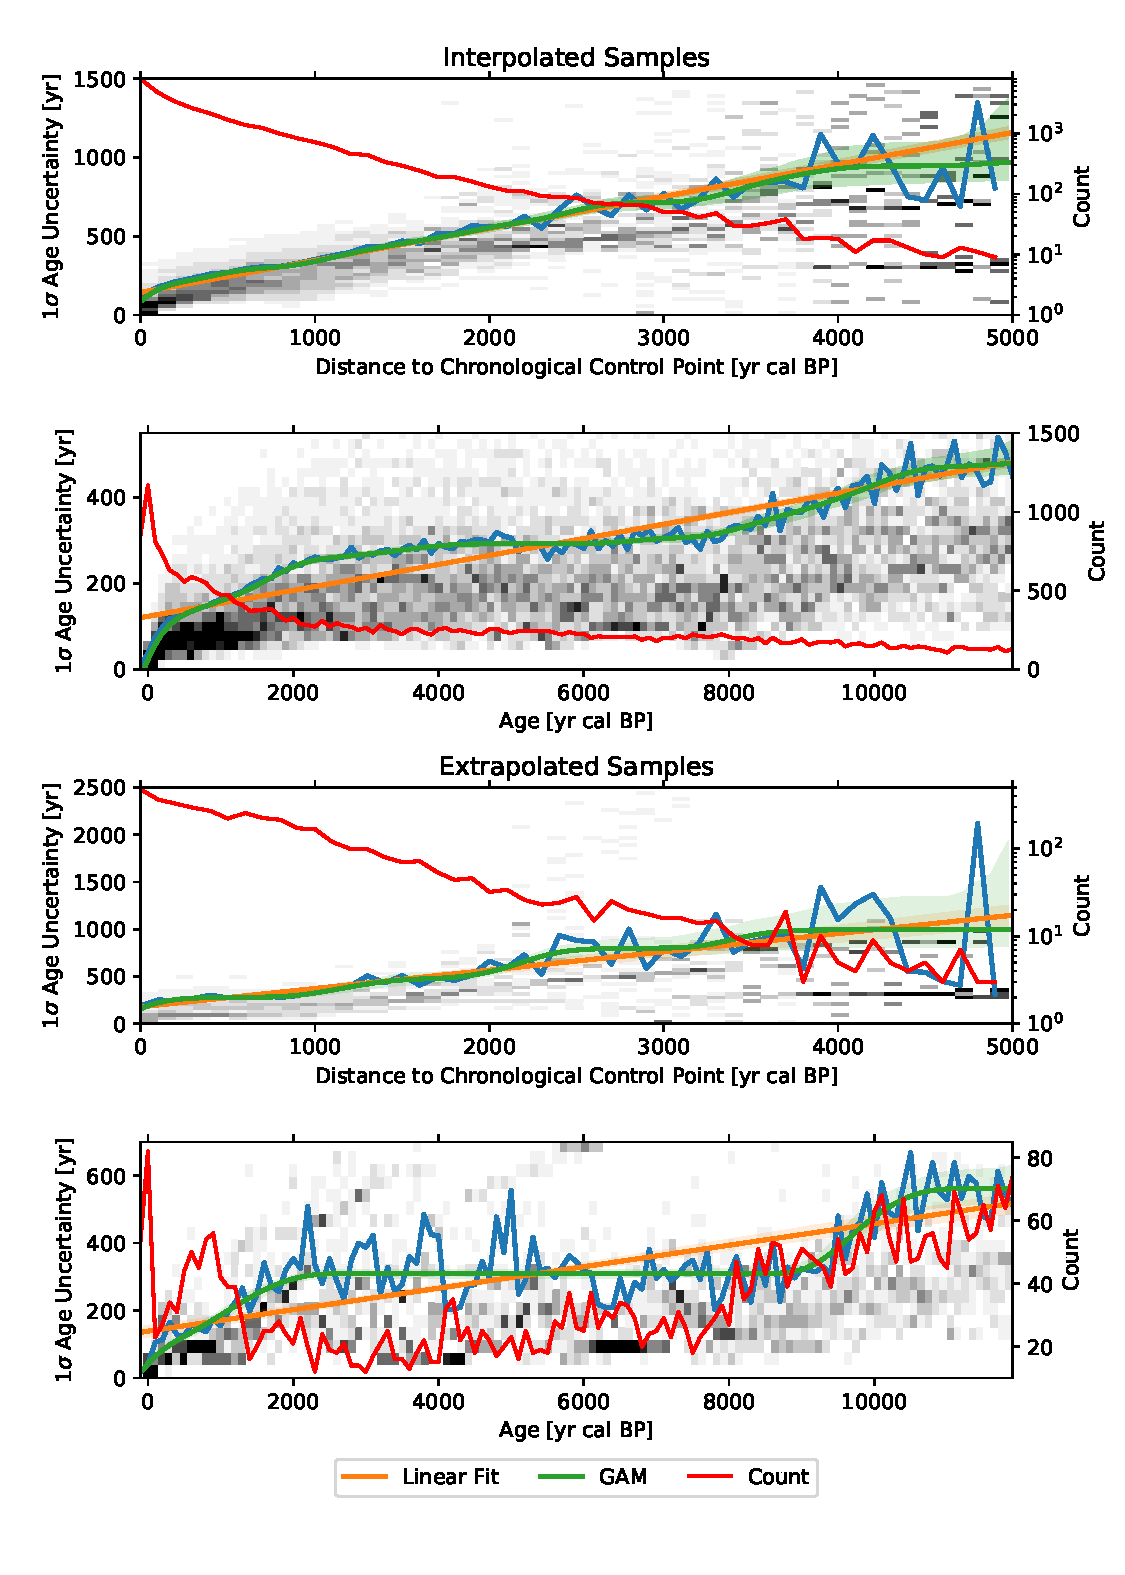
\includegraphics[width=\linewidth]{gridding-figures/univariate-models.pdf}
	\caption[Univariate age uncertainty models]{Univariate regression plots of (first and third) distance to chronological points, and (second and fourth) age to the one sigma dating uncertainty of the sample. The upper two plots contain only interpolated samples (i.e. samples that lie between two chronological control points), the lower extrapolated samples. Blue lines show the mean age uncertainty for the given distance (age). Orange and green lines show the linear and \gls{gam} fits of distance (age) to age uncertainty, and red lines show the number of samples for a given distance (age). The grayscale plot in the background shows a two-dimensional histogram (density plot) to illustrate the underlying data of the fits. For the purpose of a better visualization, each vertical bin of this histogram has been normalized to one. Means, counts and histogram are all based on 100 year bins in distance (age). The fits are estimated based on the unbinned data, the source data are all Neotoma datasets with BACON-based age-depth models. Note the logarithmic scale of the right count axis on the first and third plot.}
	\label{fig:gridding-univariate-age-unc}
\end{figure}

\begin{figure}
	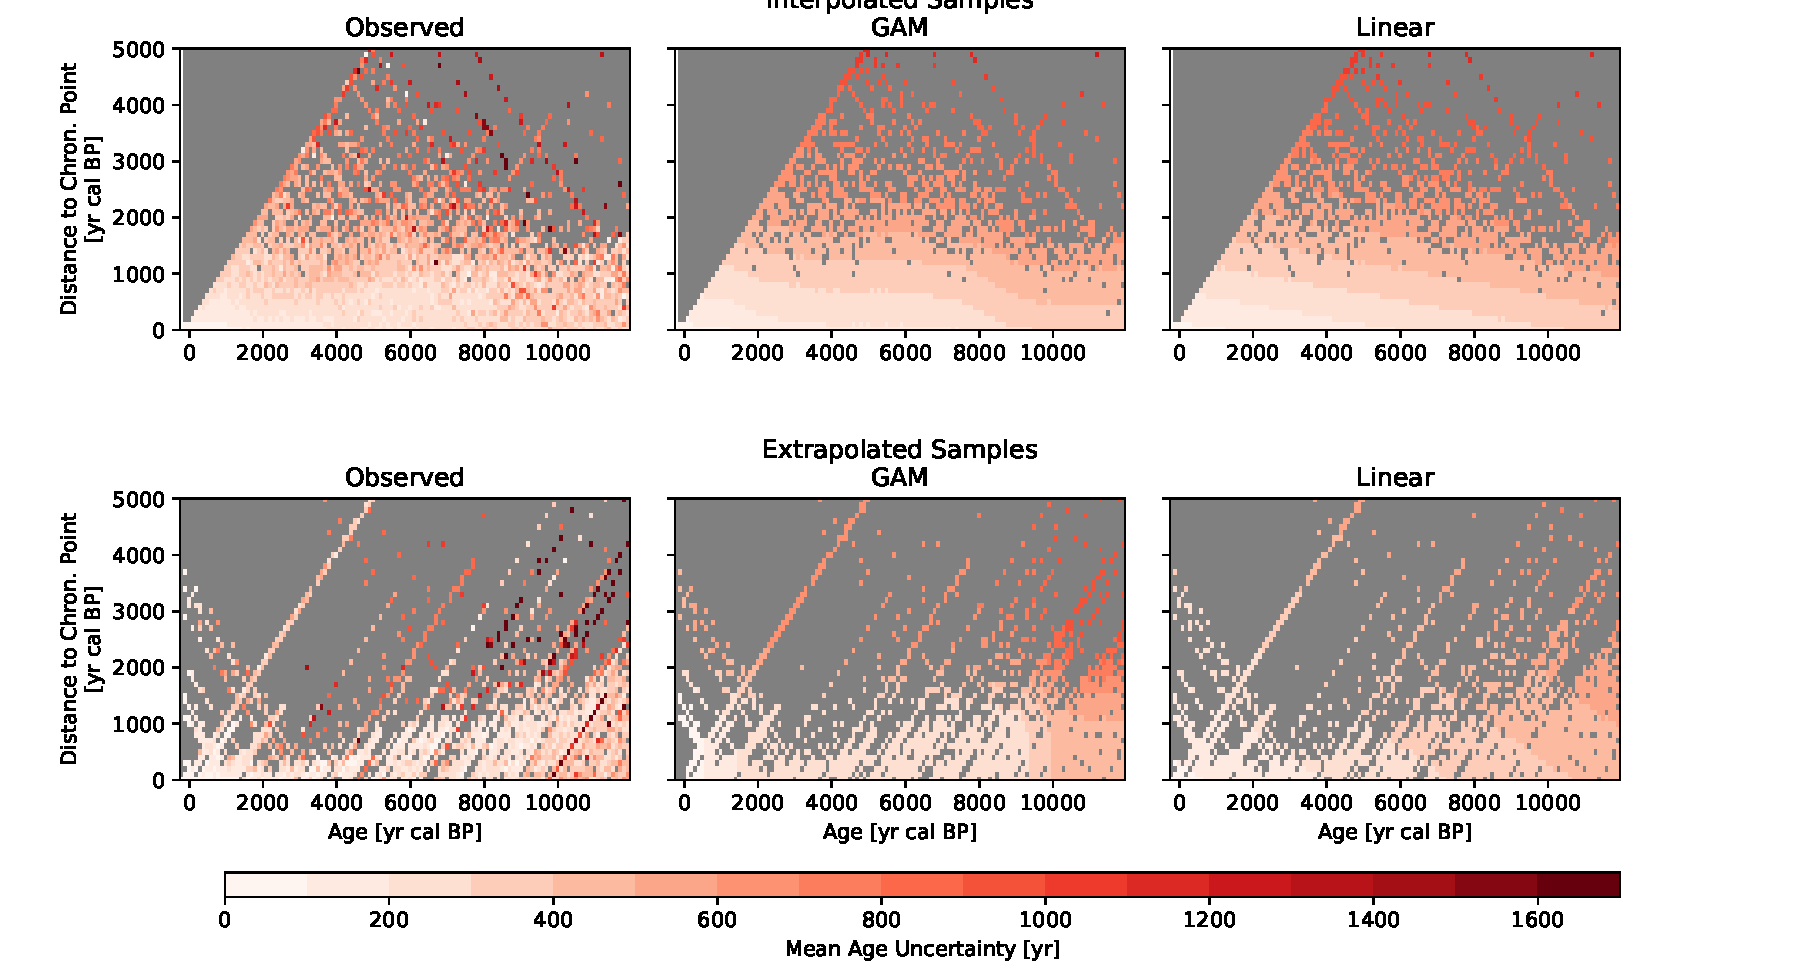
\includegraphics[width=\linewidth]{gridding-figures/bivariate-models.pdf}
	\caption[Univariate age uncertainty models]{Bivariate models of age uncertainty. Shown are the mean $1\sigma$ age uncertainties of ca. 30'000 samples from the Neotoma database sites with BACON-based age-depth models. Each sample has an age uncertainty that depends on the age of the sample (x-axis) and the distance to the closest chronological control point (y-axis). For the purpose of visualization, we grouped the samples into categories of 100 years in x- (age) and 100 years in y- (control point distance) direction, and calculated the average age uncertainty of the groups. These averages are shown with the color coding in the plots, and the gray area represents the space without any observation. The top row shows interpolated samples (i.e. samples that lie between two chronological control points), the bottom row extrapolated samples. Plots in the left column show the observed mean age uncertainties, central and right columns show the means of the predicted age uncertainties from the bivariate linear \glspl{gam} and bivariate linear regression models respectively. }
	\label{fig:gridding-bivariate-age-unc}
\end{figure}

\section{Method}  \label{sec:gridding-method}
With the intrinsic methodological uncertainties of climate and dating in mind, we present a new ensemble-based approach on gridding the reconstructions from the individual sites. Each ensemble member is generated with randomized sample ages and climate, derived from the corresponding uncertainty measures (see previous sections \ref{sec:gridding-mat} and \ref{sec:gridding-ageunc}), with additional constraints arising from the integrity of the individual dataset (sediment core). We explain these in more details in sections \ref{sec:gridding-age-sampling} and \ref{sec:gridding-temperature-sampling}. The final gridding step for each ensemble member is based on a modified setup of \cite{MauriDavisCollinsEtAl2015}, but can also be extended with other interpolation algorithms, as described in section \ref{sec:gridding-gridding}). We implemented the method as the python package \textit{pyleogrid} that efficiently scales to large datasets and ensemble sizes, and shortly describe it in section \ref{sec:gridding-package}.

\subsection{Constrained age sampling}  \label{sec:gridding-age-sampling}

\begin{figure}
	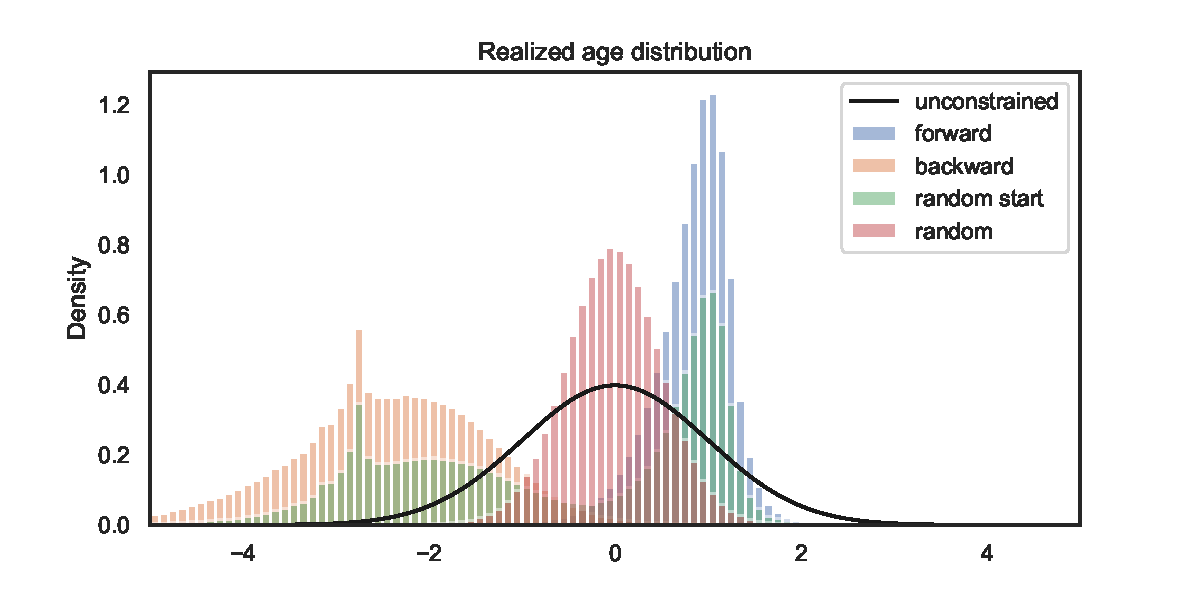
\includegraphics[width=\linewidth]{gridding-figures/age-sampling-methods-realized.pdf}
	\caption[Scaled histograms of age sampling methods]{Histograms of age sampling methods for the site in section \ref{sec:gridding-sample-site} with an ensemble size of 10'000. Every sampled age has been centered at the reported age of the corresponding sample and scaled by its age uncertainty. The black line shows the unconstrained distribution (a standard normal with a standard deviation of 1), the other histograms show the realized distributions for each of the age sampling methods (section \ref{sec:gridding-age-sampling}). Note that \textit{random sort} and \textit{Gibbs} histograms highly overlap.}
	\label{fig:gridding-age-sampling-methods}
\end{figure}

Every dataset has an intrinsic monotonicity constraint that the sample deeper down the core has an older age. An inversion of this constraint is very rare and is usually visible in the stratigraphy of the core, such that affected samples are ruled-out before. As such, a classic unconstrained sampling of ages\footnote{\label{foot:unconstrained-note}We call it the unconstrained distribution for convenience, but keeping in mind that every sampled age has to be older than -70 yr cal BP.} using a normal distribution centered at reported sample age and a scale corresponding to the estimated age uncertainty (section \ref{sec:gridding-ageunc}) violates this constraint. Samples are inverted in such a case when their uncertainty intervals overlap and as such the individual ensemble member would not maintain the integrity of the individual core. We illustrate an example for such a core in section \ref{sec:gridding-site}.

\textit{pyleogrid} therefore implements different variants of this constraint with the Gibbs sampling being the one that is finally used.

\subsubsection{The intuitive approach}
The most intuitive approach is to randomly draw a sample age and constraint the age of the neighboring sample with it. This can be done in a \textit{forward} manner, such that every older sample has to be older than the previous younger sample, or in a backward manner, i.e. the younger sample has to be younger than the neighboring older sample. We will show in the paragraphs below that this method is biased, nevertheless we mention it here because of the intuitivity of the approach and because the reason for the failure is non-trivial.

As such, we demonstrate three different algorithms:

\begin{description}
	\item[forward] Starting with an unconstrained age distribution for the youngest sample in the core, every consecutive sample has to be older than the previous (i.e. the method works forward in age, but backward in time
	\item[backward] Starting with an unconstrained age distribution for the oldest sample in the core, every consecutive sample has to be younger than the previous (i.e. the method works backward in age, but forward in time)
	\item[random start] Starting with an unconstrained age distribution of a random sample in the core, we apply the \textit{backward} algorithm for younger and \textit{forward} algorithm for younger samples.
\end{description}

As such, \textit{forward} and \textit{backward} algorithms always start with an unconstrained age distribution of the youngest (oldest) sample for every ensemble member. Within the \textit{random start} algorithm, every sample gets the chance to start with an unconstrained age distribution, because the starting point is random for every ensemble member. The constrained age distributions for the consecutive samples are implemented as truncated normal distributions.

The resulting age distributions from the three algorithms are shown in figure \ref{fig:gridding-age-sampling-methods}, together with another method, that is described later in this section. The figure shows the sampled age distributions by the various above-mentioned sampling methods for the site described in section \ref{sec:gridding-sample-site}. To make these age distributions comparable, we transformed them to a standard normal distribution (visualized as the unconstrained distribution in figure \ref{fig:gridding-age-sampling-methods}) prior to visualization, by subtracting the reported age and dividing by the estimated age uncertainty of the corresponding sample. It is obvious from this figure that all of the above-mentioned algorithms produce an artificial bias to the age distribution. The \textit{forward} approach pushes the samples to the upper tail of the distribution, the \textit{backward} approach pushes everything to the lower tail. The \textit{random start} method produces a bimodal distribution with peaks at the upper and lower tail.

This is also shown with three exemplary samples from the site in the supplementary figure \ref{fig:gridding-age-example-distributions}. The forward method works well for the young sample but pushes all older samples to the upper tail of their distribution, The backward method does the opposite and the random sort method creates a bimodal distribution for the sample in the center of the core, and backward behaves like the forward (backward) algorithm at the older (younger) part of the core.

We explain this initially unexpected results with the overlapping age uncertainties in the core. The site that we describe here has 110 samples. As such, the probability that one sample draws a random age at the lower or upper tail of the distribution is very high. Now, most of the dating uncertainty intervals overlap and this forces all the consecutive samples to the tail of their age distributions. Another problem, that is not shown here, arises from the differing sizes of the age uncertainties which highly depends on the distance to the chronological control point (see section \ref{sec:gridding-ageunc}). This can also lead to unsatisfiable requirements, if one sample is close to a control point (and as such has a lower age uncertainty) and the previous sample has been pushed far outside of the 95\% confidence interval.


\subsubsection{The random sorting approach}

These strong biases of the intuitive approach led to another method, that we also show in red in figure \ref{fig:gridding-age-sampling-methods} and supplementary figure \ref{fig:gridding-age-example-distributions}, the \textit{random sort} method. This method consists of two steps: in the first step we draw random age for each sample based on its unconstrained distribution\textsuperscript{\ref{foot:unconstrained-note}}. In the second step, we order these random ages while maintaining the order of samples in each dataset. As such, we assign an age to each sample that is not necessarily drawn from its own distribution, but rather from the one of a neighboring sample. When samples overlap, this then truncates the tails of realized distribution and effectively decreases the reported age uncertainty, as can be seen in the figures \ref{fig:gridding-age-sampling-methods}, \ref{fig:gridding-age-example-distributions}. This approach is mathematically difficult to justify because it violates the common methodology that each sample has a unique confidence interval that it needs to explore. Therefore the method might introduce some hidden biases in the sampled distributions that are difficult to quantify. Nevertheless, the algorithm is very fast and much closer to the desired joint distribution, than the previous \textit{intuitive} approach. But in order to avoid any biases and to guarantee a mathematically correct result, we chose to implement a Gibbs sampling algorithm to sample from the desired constrained distribution.


\subsubsection{The Gibbs sampling approach}

\begin{figure}
	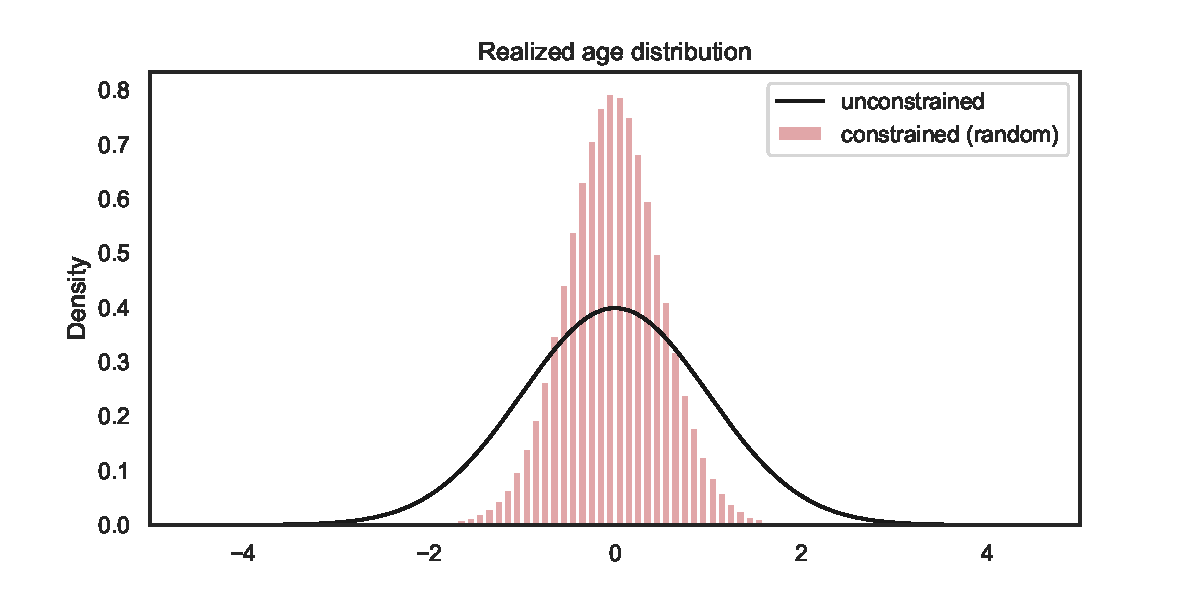
\includegraphics[width=\linewidth]{gridding-figures/full-realized-age-distribution.pdf}
	\caption[Realized age distribution for the entire dataset]{Realized age distribution for the entire dataset (section \ref{sec:gridding-polnet}) with the \textit{random} method (section \ref{sec:gridding-age-sampling}). The individual sample distributions have been centered and scaled as in figure \ref{fig:gridding-age-sampling-methods}.}
	\label{fig:gridding-full-age-distribution}
\end{figure}

\begin{algorithm}[h]
\renewcommand{\algorithmicensure}{\textbf{Output:}}
\caption[Accept/Reject algorithm]{Accept/Reject algorithm. $\mathcal{N}(\mu, \sigma)$ denotes the normal distribution with location parameter $\mu$ and shape parameter $\sigma$.}
\label{a:gridding-mcmc}
\begin{algorithmic}[1]
	\STATE Set $i = 0$
	\STATE Set $\boldsymbol{\mu}$ as vector of the reported ages in $dataset$
	\STATE Set $\boldsymbol{\sigma}$ as vector of estimated age uncertainties		
	\STATE Set $\mathbf{a}$ (the target age vector) to be of length $\boldsymbol{\mu}$
	\WHILE{$i < 1$ \OR \NOT $is\_monotonic(\mathbf{a})$}
	\STATE $\mathbf{a} = \mathcal{N}(\boldsymbol{\mu}, \boldsymbol{\sigma}^2)$
	\STATE Set $i = i + 1$
	\ENDWHILE
\end{algorithmic}
\end{algorithm}

The biases of the above-mentioned algorithms led to the development of a \gls{mcmc} sampling algorithm. An accept/reject algorithm which draws a set of random ages for all unconstrained sample distributions in a core at once and accepts the draw if the monotonicity condition is satisfied and rejects the sample if the monotonicity condition was initially explored. For one realization of the ages $\mathbf{a}$ in a given dataset, this is described with the pseudo-code in algorithm \ref{a:gridding-mcmc}. This standard approach however did not find a monotonic solution within ten million iterations for a high-resolution site such as it has been used in the previous section. 

Therefore we decided to implement a Gibbs sampler, an algorithm that is commonly used in Bayesian inference to obtain a sequence of samples from conditional probability distributions, which generate samples from a multivariate joint distribution when this distribution is unknown and/or cannot be sampled directly. In our case, this distribution if the distribution of all sample ages in one dataset, where each sample age is conditioned by it's younger and older neighbor. Let $\boldsymbol{\mu} = \left(\mu_1, \mu_2, \ldots \mu_N \right)$ be the reported ages of the $N$ pollen samples in one individual dataset with estimated age uncertainties $\boldsymbol{\sigma} = \left(\sigma_1, \sigma_2, \ldots \sigma_N \right)$. The reported ages fulfill the monotonicity constrain, i.e. $\mu_j \leq \mu_k$ for all $j, k$ with $1 \leq j \leq k \leq N$. The objective of our sampling approach is to generate $M$ random realizations of $\boldsymbol{\mu}$, denoted by $\mathbf{X}^{(m)} = \left(X^{(m)}_1, X^{(m)}_2, \ldots X^{(m)}_N \right)$ with $m=1,\ldots,M$, that all fulfill the monotonicity constrain. In other words, the realizations $\mathbf{X}^{(m)}$ are constrained to fulfill

\begin{equation}
	X^{(m)}_j \leq X^{(m)}_k, \text{ for all } j, k \text{ with } 1 \leq j \leq k \leq N \text{ and } 1\leq m \leq M.
\end{equation}

We set the intial value to the reported ages ($\mathbf{X}^{(1)} = \boldsymbol{\mu}$) where we know that the constrain is fullfilled. For the following realizations $\mathbf{X}^{(m+1)}$ with $1 < m \leq M$ we sample each component $X_j^{(m)}$ with $1 \leq j \leq N$ conditioned by its previous sample $X_{j-1}^{(m)}$ and, most importantly, conditioned by the next sample, but from the previous realization, i.e. $X_{j+1}^{(m-1)}$. As such, we define the sampled age of $X_j^{(m)}$ with

\begin{equation}
	X^{m}_j = \mathcal{N}(X_{j-1}^{(m)}; X_{j+1}^{(m-1)}; \mu_j, \sigma_j^2)
\end{equation}

where $\mathcal{N}(a; b; \cdot, \cdot)$ denotes a random variate of the truncated normal distribution with lower limit $a$ and upper limit $b$. Although this algorithm always starts with the youngest sample in the dataset for every realization, such as the \textit{forward} method, it does not push every sample to the lower tail of the distribution because every sampled age is conditioned by the age of the next pollen sample from the previous realization. It is mathematically proven that the combined realizations $\left\lbrace\mathbf{X}^{(1)}, \mathbf{X}^{(2)}, \ldots \mathbf{X}^{(M)}\right\rbrace$ of this algorithm approximates the joint distribution of the sample ages in the dataset under the given constraint, and that each marginal distribution of a the age of a particular pollen sample $1 \leq j \leq N$ is approximated by $\left\lbrace X_j^{(1)}, X_j^{(2)}, \ldots, X_j^{(M)} \right\rbrace$.

As it is common for a \gls{mcmc} algorithm, each realization is correlated with nearby realizations. The first samples are particularly correlated with the initial value $\boldsymbol{\mu}$ and it is therefore common practice to discard the first 1000 realizations, the so-called \textit{burn-in} period. 

To avoid an autocorrelation between the successive realizations, we \textit{thin} our set of sampled ages and keep only every tenth realization until we have the desired amount of $M$ realizations. The value of 10 has been shown to be sufficient using an autocorrelation analysis of the different samples in the Tigalmamine record.

As can be seen in figure \ref{fig:gridding-age-sampling-methods} and \ref{fig:gridding-age-example-distributions}, the outcomes are very close to the above mentioned \textit{random sort} approach. However, a look into the realized distribution of the last sample in figure \ref{fig:gridding-age-example-distributions} reveals a negative bias of the distribution sampled with the \textit{random sort} approach.

The realized (and standardized) distribution of the entire database presented in section \ref{sec:gridding-polnet} is finally shown in figure \ref{fig:gridding-full-age-distribution}. The comparison with the unconstrained distribution in this figure highlights the need for a constrained sampling because the latter significantly reduces the width of the distribution.

\subsection{Temperature sampling}  \label{sec:gridding-temperature-sampling}

\begin{figure}[h]
	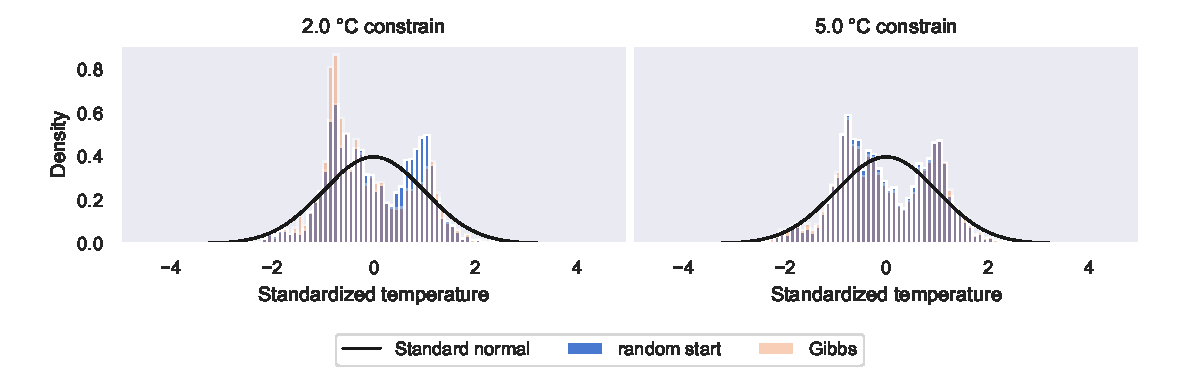
\includegraphics[width=\linewidth]{gridding-figures/temp-sampling-methods-realized.pdf}
	\caption[Scaled histograms of temperature sampling methods]{Histograms of temperature sampling methods for the site in section \ref{sec:gridding-sample-site} with an ensemble size of 10'000 for a climatic constraint of (left) 2 °C, and (right) 5 °C. As in figure \ref{fig:gridding-age-sampling-methods}, every sampled temperature has been centered at the weighted average of the corresponding modern analogues and scaled by the corresponding weighted standard deviation. The black line shows the unconstrained distribution (a standard normal with a standard deviation of 1), the other histograms show the realized distributions for \textit{random start} and \textit{Gibbs} temperature sampling method (section \ref{sec:gridding-age-sampling}).}
	\label{fig:gridding-temp-sampling-methods}
\end{figure}

\begin{figure}[!t]
	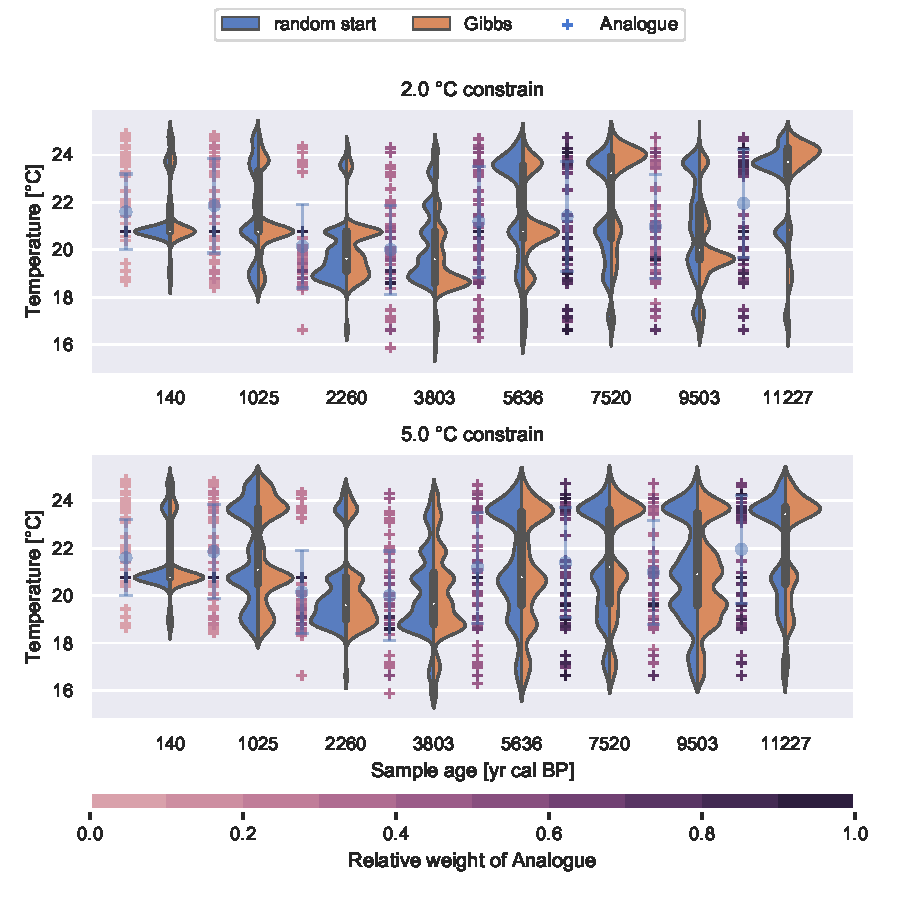
\includegraphics[width=\linewidth]{gridding-figures/tigal-sample-climate-violins.pdf}
	\caption[Realized temperature distributions for a few samples]{Violin plots for sampled temperature distributions of some samples in the Tigalmamine record with a climatic threshold of (top) 2 and (bottom) 5 °C. Blue (left) distributions are realized with the \textit{random start} method, ocher (right) areas with Gibbs sampling. The crosses to the left of each violin shows the locations of the climate analogues. Each cross is color coded by it's chord distance relative to the chord distance of the closest analogue (i.e. the closest analogue has always a weight of 1).}
	\label{fig:gridding-temp-sampling-violins}
\end{figure}

As already mentioned in \ref{sec:gridding-mat}, our sampling approach does not use the temperature and uncertainty reported for every single variable. Instead, it samples the underlying distribution. As such, our method can be adapted to multiple site-specific reconstruction methods, such as weighted averaging (WA), weighted-averaging partial-least squares (WAPLS) \citep{BirksBraakLineEtAl1990, BraakJuggins1993} or other approaches \citep[e.g.][]{BirksHeiriSeppaeEtAl2010, BrewerGuiotBarboni2007, Juggins2013}. In this study, we use a \gls{mat} approach (see section \ref{sec:gridding-mat}) and sample the discrete set of climate analogues for each sample. The probability to select an analogue (i.e. it's weight) is thereby determined by the chord distance between the fossil and modern pollen assemblages. The closer the assemblages (relative to the other potential analogues), the higher the weight.

This methodology is substantially different from the standard approach, such that is takes the multimodality of the analogues into account, whereas the standard appraoch (weighted average of the $k$ closest analogues) estimates a unimodal distribution. It additionally better represents the discrete nature of the analogue approach whereas the standard method intrinsically assumes a continuity in the distribution. In fact, only a small part of the available climate space is actually represented by the modern analogues. The 5'500 modern analogues for Tigalmamine, for instance (110 samples with 50 analogues each), are represented by only 240 distinct modern pollen samples with only 131 distinct \gls{jja} temperatures and they eventually span a large climate space (see figure \ref{fig:gridding-site-analogues}).

The latter gives the motivation for a climatic constraint that ensures the integrity of the individual dataset. It is, for instance, impossible that two samples from the same dataset but 200 years apart experience a temperature difference of five degrees or more between each other. This is, however, a possible combination, considering the underlying set of analogues (see figure \ref{fig:gridding-site-analogues} for instance). We therefore perform a constrained sampling, as in section \ref{sec:gridding-age-sampling}, and implement a fixed temperature threshold $T$. Every sampled analogue in each dataset (i.e. every choice of the discrete distribution for each pollen sample) is constraint to not differ by more than $T$ degrees celsius from its temporally neighboring samples. The exact choice of $T$ is a critical assumption and has a major impact on the realized temperature distribution for each sample. We decided for a very conservative estimate of five degrees, which is only applied if the samples do not differ by more than 1000 years. These choices are further discussed in section \ref{sec:gridding-results}.

In the remainder of this section, we focus on the implementation of this conditional sampling, because of its substantial impact on the realized distribution, as already shown for the sampled ages in section \ref{sec:gridding-age-sampling}. We briefly discuss the same approaches as in section \ref{sec:gridding-age-sampling} (without the \textit{random sort} algorithm because we do not enforce monotonicity here). The core of the method is the same for all approaches: If a climate analogue differs by more than $T$ degrees from the temperature of the conditioning sample, its probability is set to zero. The choice about the \textit{conditioning sample} is dependent on sampling algorithm. Here, we discuss following methods:

\begin{description}
	\item[forward] The temperature of every older sample must not differ by more than $T$ from its younger sample
	\item[backward] The temperature of every younger sample must not differ by more than $T$ from its older sample
	\item[random start] Starting with a random sample in a data, we apply the forward method to older and the backward method to younger samples
	\item[Gibbs] The choice for each sample is constrained by the younger sample and the older sample from the previous realization of the dataset.
\end{description}

We described these algorithms already in detail in section \ref{sec:gridding-age-sampling} and therefore focus only on the comparison of results. The only difference is that now, without the monotonicity constraint, \textit{forward} and \textit{backward} methods give the same result as the \textit{random start} method. Therefore we will only focus on the last two methods.

Figure \ref{fig:gridding-temp-sampling-methods} shows the realized distributions for the two methods. As in the corresponding figure for the age sampling (figure \ref{fig:gridding-age-sampling-methods}), we subtracted the weighted average of the climate analogues of the corresponding pollen sample by each of the randomly sampled temperature values, and afterwards divided by the weighted standard deviation, in order to make the drawn temperature values at the different ages comparable. Both methods realize a bimodal distribution (a feature that is also visible in the spread of the climate analogues in figure \ref{fig:gridding-site-analogues}) and result in the similar distributions when considering a climate constraint of 5 °C. This does not hold for the stronger 2 °C constraint, where the Gibbs method gives more weight to samples below the weighted average. This is caused by the additional constraint of the Gibbs sampling approach where each sample is constrained by the sample of the previous realization. The algorithm always starts with the youngest sample which has a higher probability in the Moroccan regime (green area, figure \ref{fig:gridding-site-analogues}). Due to the constraint of the sample in the previous realization, it then is more likely that we stay in this regime. As such, the distribution tends to get more unimodal compared to the other method, where each realization is entirely independent of the other.

This difference between the two methods and the two climatic constraints is further illustrated in figure \ref{fig:gridding-temp-sampling-violins}, which shows the violin plots for a selection of samples in the Tigalmamine record, separated by method and climatic constraint. As already shown with the standardized temperatures in figure \ref{fig:gridding-temp-sampling-methods}, the two methods are approximately equal under the 5 °C constraint and significantly reduce the realized temperature regime with a more multimodal distribution under the 2 °C constraint. The Gibbs method tends to sharpen the distribution at the locations of the analogue climates stronger than the \textit{random start} method, which implies that the latter is again prone to (potentially) large and unknown biases. 

\subsection{Gridding}  \label{sec:gridding-gridding}

\begin{figure}
	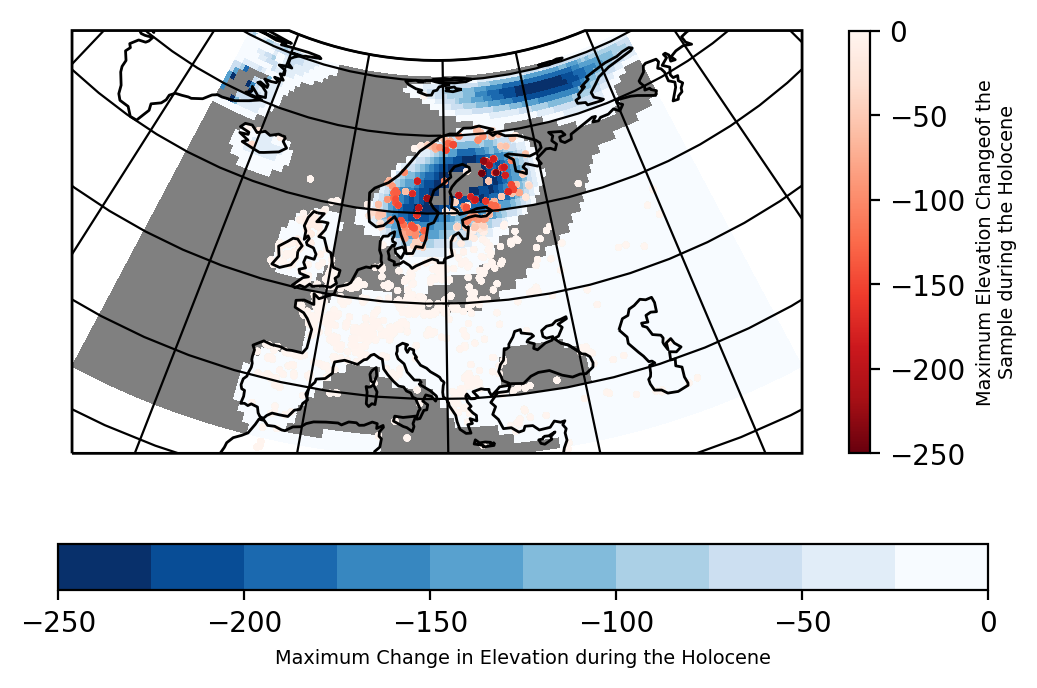
\includegraphics[width=\linewidth]{gridding-figures/elevation-difference.png}
	\caption[Elevation difference and corrections]{Maximum change of elevation during the Holocene per grid cell (blue background), based on the data from the ICE-6G model. The dots show the applied (maximal) corrections to the samples in these locations. \todo[inline, size=\normalsize]{Elevation figure has to be made nicer.}}
	\label{fig:gridding-elev-correction}
\end{figure}

\begin{figure}
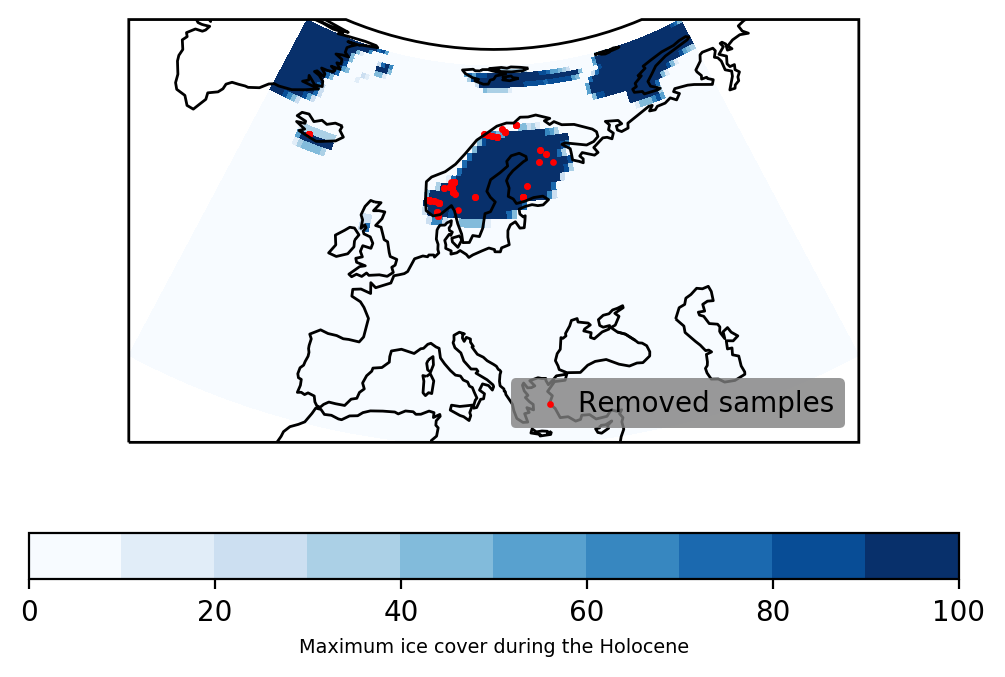
\includegraphics[width=\linewidth]{gridding-figures/elevation-mask.png}
\caption[Ice sheet mask of the pollen samples]{Locations of samples (red dots) that have been removed from the input data because they are covered by ice (according to the ICE-6G model, blue background). \todo[inline, size=\normalsize]{ice sheet mask has to be made nicer.}}
\label{fig:gridding-elev-mask}
\end{figure}

The underlying gridding algorithm is the same as in \cite{MauriDavisCollinsEtAl2015}, the thin plate spline regression method (\textit{Tps}) of the \textit{fields} R-package \citep{NychkaFurrerPaigeEtAl2017, RCT2019}. This method interpolates the scalar variable (temperature) from the irregularly spaced four dimensional sample data onto a two dimensional surface (defined by latitude, longitude and elevation) in 3D space. The time component is considered by giving a higher weight to samples that are temporally closer to the target time of the interpolation.

The major difference compared to \cite{MauriDavisCollinsEtAl2015} is the ensemble approach, which can also be interpreted as a bootstrapping approach. We apply the gridding many times to different realizations of the input data. The major advantage of this ensemble approach is the sophisticated distribution of temperatures per grid cell. This allows a better estimate of the uncertainty of the gridded climate reconstruction, compared to \cite{MauriDavisCollinsEtAl2015}. But it should be noted that this ensemble approach is structurally independent of the underlying regression algorithm. Hence, it can potentially also be extended to other gridding methods.

Another difference between our study and \cite{MauriDavisCollinsEtAl2015} is the type of climatic variable. \cite{MauriDavisCollinsEtAl2015} calculated interpolated anomalies, whereas we interpolate the absolute climate climate variable as it is derived from the pollen-climate reconstruction method. The advantage is that we can directly interpolate to the elevation at a given timestep, whereas \cite{MauriDavisCollinsEtAl2015} applied an a posteriori isostatic correction. 

For the reconstruction presented in section \ref{sec:gridding-results}, we use the data of the ICE-6G-C model \citep{ArgusPeltierDrummondEtAl2014, PeltierArgusDrummond2015}, that is also used in the PMIP4 experiments \citep{IvanovicGregoireKageyamaEtAl2016, Otto-BliesnerBraconnotHarrisonEtAl2017, KageyamaBraconnotHarrisonEtAl2018}. To account for the change in elevation, \textit{pyleogrid} also implements a method to correct the elevation of the samples based on the elevation difference in the given input raster for the different time steps. The results of this correction can be seen in figure \ref{fig:gridding-elev-correction}. In addition to this elevation correction, we removed samples from the input data where the ICE-6G model reports an ice coverage of more than 50\% in the grid cell (figure \ref{fig:gridding-elev-mask}). Affected samples are all during the early Holocene in northern Europe.

\subsection{Implementation}  \label{sec:gridding-package}
The ensemble method presented in this thesis is available as the python package \textit{pyleogrid} from \href{https://github.com/Chilipp/pyleogrid}{github.com/Chilipp/pyleogrid} \todo{add DOI}. The documentation of the package is available at \href{https://pyleogrid.readthedocs.io}{pyleogrid.readthedocs.io}. This module also contains the models for predicting age uncertainties (section \ref{sec:gridding-ageunc}), that are based on the \textit{pyGAM} software \citep{ServenBrummittAbedi2018}. The github repository and the documentation contains the notebooks that are used to run the analysis of this study.

The sampling methods of \textit{pyleogrid} that generate entirely independent realizations of the input data (forward, backward, random start and random sort methods) are built using the functionalities of the numerical numpy and scipy packages \citep{Oliphant2006, JonesOliphantPetersonEtAl2001} to efficiently generate thousands of constrained realizations of the input data. The computationally more expensive Gibbs sampling algorithms (section \ref{sec:gridding-age-sampling} and \ref{sec:gridding-temperature-sampling}) were every realization is constrained by the previous realizations, is implemented in Cython \citep{BehnelBradshawCitroEtAl2011}, an optimising static compiler for Python, and uses the corresponding Cython \glspl{api} of numpy and scipy.

As already mentioned in section \ref{sec:gridding-gridding}, \textit{pyleogrid} uses the \textit{Tps} method of the \textit{fields} package \citep{NychkaFurrerPaigeEtAl2017} and as such interfaces into an R environment for the gridding.

\textit{pyleogrid} is designed to scale to large amounts of input data (e.g. for a global reconstruction or hemispheric reconstruction) on a local computer or a large parallelized cluster, using the xarray and dask packages for parallel computing and out-of-core computation \citep{HoyerHamman2017, DDT2016}.

\section{Results}  \label{sec:gridding-results}
In this section we briefly present the results of the final temperature reconstruction, both for the site-based reconstruction at Tigalmamine (section \ref{sec:gridding-site}), and the western Eurasian gridded temperature record for selected time slices (section \ref{sec:gridding-gridded-results}). The purpose of this section is present the results of the ensemble approach with a special focus on the choices that have been made in the methods section, particularly the number of analogues and the climatic constraint. We focus on the ensemble mean, but it is important to keep in mind that our method approximates the joint spatio-temporal distribution of the climate.

\subsection{Site-based realized climate reconstruction: a use-case} \label{sec:gridding-site}

\begin{figure}
	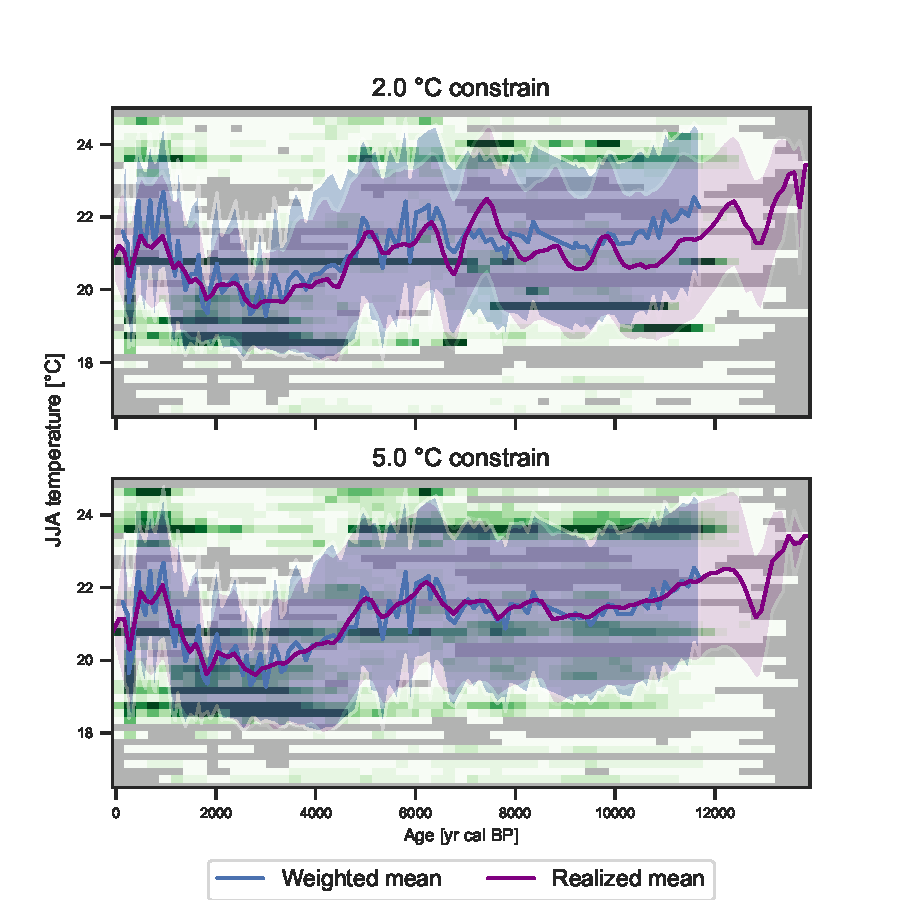
\includegraphics[width=\linewidth]{gridding-figures/realized-temperature-tigalmamine.pdf}
	\caption[Realized summer temperature reconstruction of Tigalmamine with different constraints]{Realized summer temperature reconstruction of Tigalmamine from the Gibbs sampling with a temperature constraint of (top) 2 °C and (bottom) 5 °C. The background shows a density plot of the sampled age-temperature pairs within the ensemble of 10'000 realizations. The purple line is the mean of all sampled temperatures within 100-year bins, i.e. it represents the mean of the marginal temperature distribution at a given age. The blue curve is the weighted average of the standard \gls{mat} approach (black dashed line in figure \ref{fig:gridding-site-analogues}). The shaded areas correspond to the standard deviations of the corresponding line.}
	\label{fig:gridding-tigal-recon}
\end{figure}

\begin{figure}
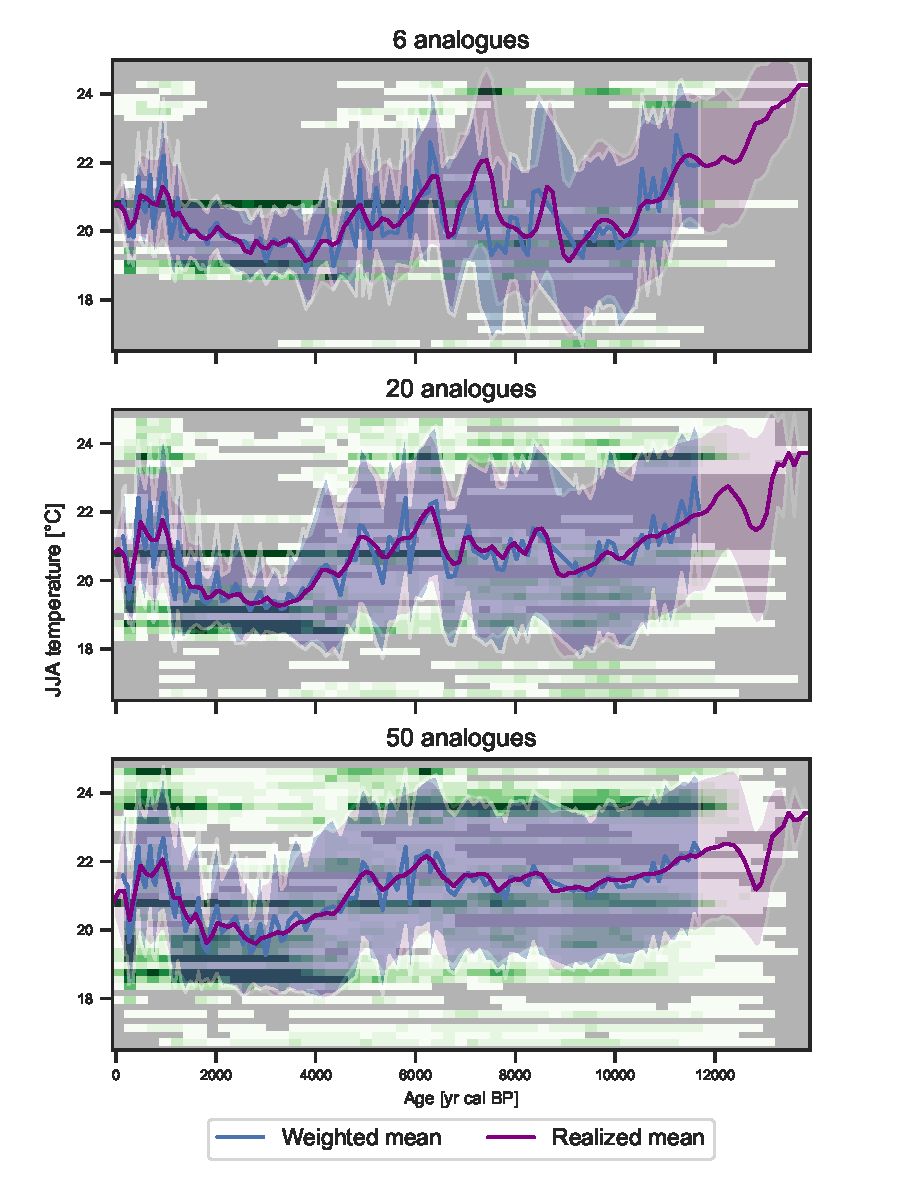
\includegraphics[width=\linewidth]{gridding-figures/realized-temperature-tigalmamine-kanalogues.pdf}
\caption[Realized summer temperature reconstruction of Tigalmamine with different analogues]{Realized summer temperature reconstruction of Tigalmamine from the Gibbs sampling with 5 °C constraint for (top) 6 analogues, (middle) 20 analogues and (bottom) the default 50 analogues. The weighted means (blue curves) have been calculated using only the 6, 20 or 50 analogues. See figure \ref{fig:gridding-tigal-recon} for a description of the elements in the plot.}
\label{fig:gridding-tigal-recon-k}
\end{figure}

The final reconstruction of the Tigalmamine site for an ensemble size of 10'000 realizations is displayed in figure \ref{fig:gridding-tigal-recon}. It shows a density plot of the realized temperature and age regime, as well as the weighted average of the \textit{standard approach}. For comparison we also show the mean of the marginal temperature distribution record from our method (we call this the \textit{realized mean} from now). The plot shows how our method realizes the site within the ensemble. It shows the \textit{Moroccan} regime during the late Holocene (lower left dark green area between 0 and 4'000 years cal BP, see also figure \ref{fig:gridding-site-analogues}) and the \textit{Spanish} regime during the early to mid Holocene (upper right dark green area in figure \ref{fig:gridding-tigal-recon}). The figure also displays the differences between the two temperature constraints. As already mentioned in section \ref{sec:gridding-temperature-sampling}, the 2 °C constraint results in a more multimodal distribution, especially towards the end of the record. The the realized mean is therefore significantly different from the weighted average of the standard approach. 

Figure \ref{fig:gridding-tigal-recon-k} shows the same figure but for a varying number of analogues. The trends of the three images behave the same and show all a decrease in temperature during the early holocene and a small plateau during the last millenium. Also the temperature regimes conform with a the above-mentioned dominance of the \textit{Moroccan regime} in the late Holocene the \textit{Spanish regime} during the early Holocene. With a lower number of analogues, however, (top plot) the temperature changes in the means are much smaller over a short period of time. The distribution for this scenario (green 2D histgram in the plot) shows a strong multimodality with a few temperature values that have a very high probability. The scenarios with higher analogues (20 or 50) result in a much smoother mean because the underlying distribution covers more of the available age-temperature space.

\subsection{Gridded summer temperature} \label{sec:gridding-gridded-results}

\subsubsection{Determinstic vs. ensemble approach}

\begin{figure}
	\captionsetup{width=\linewidth}
	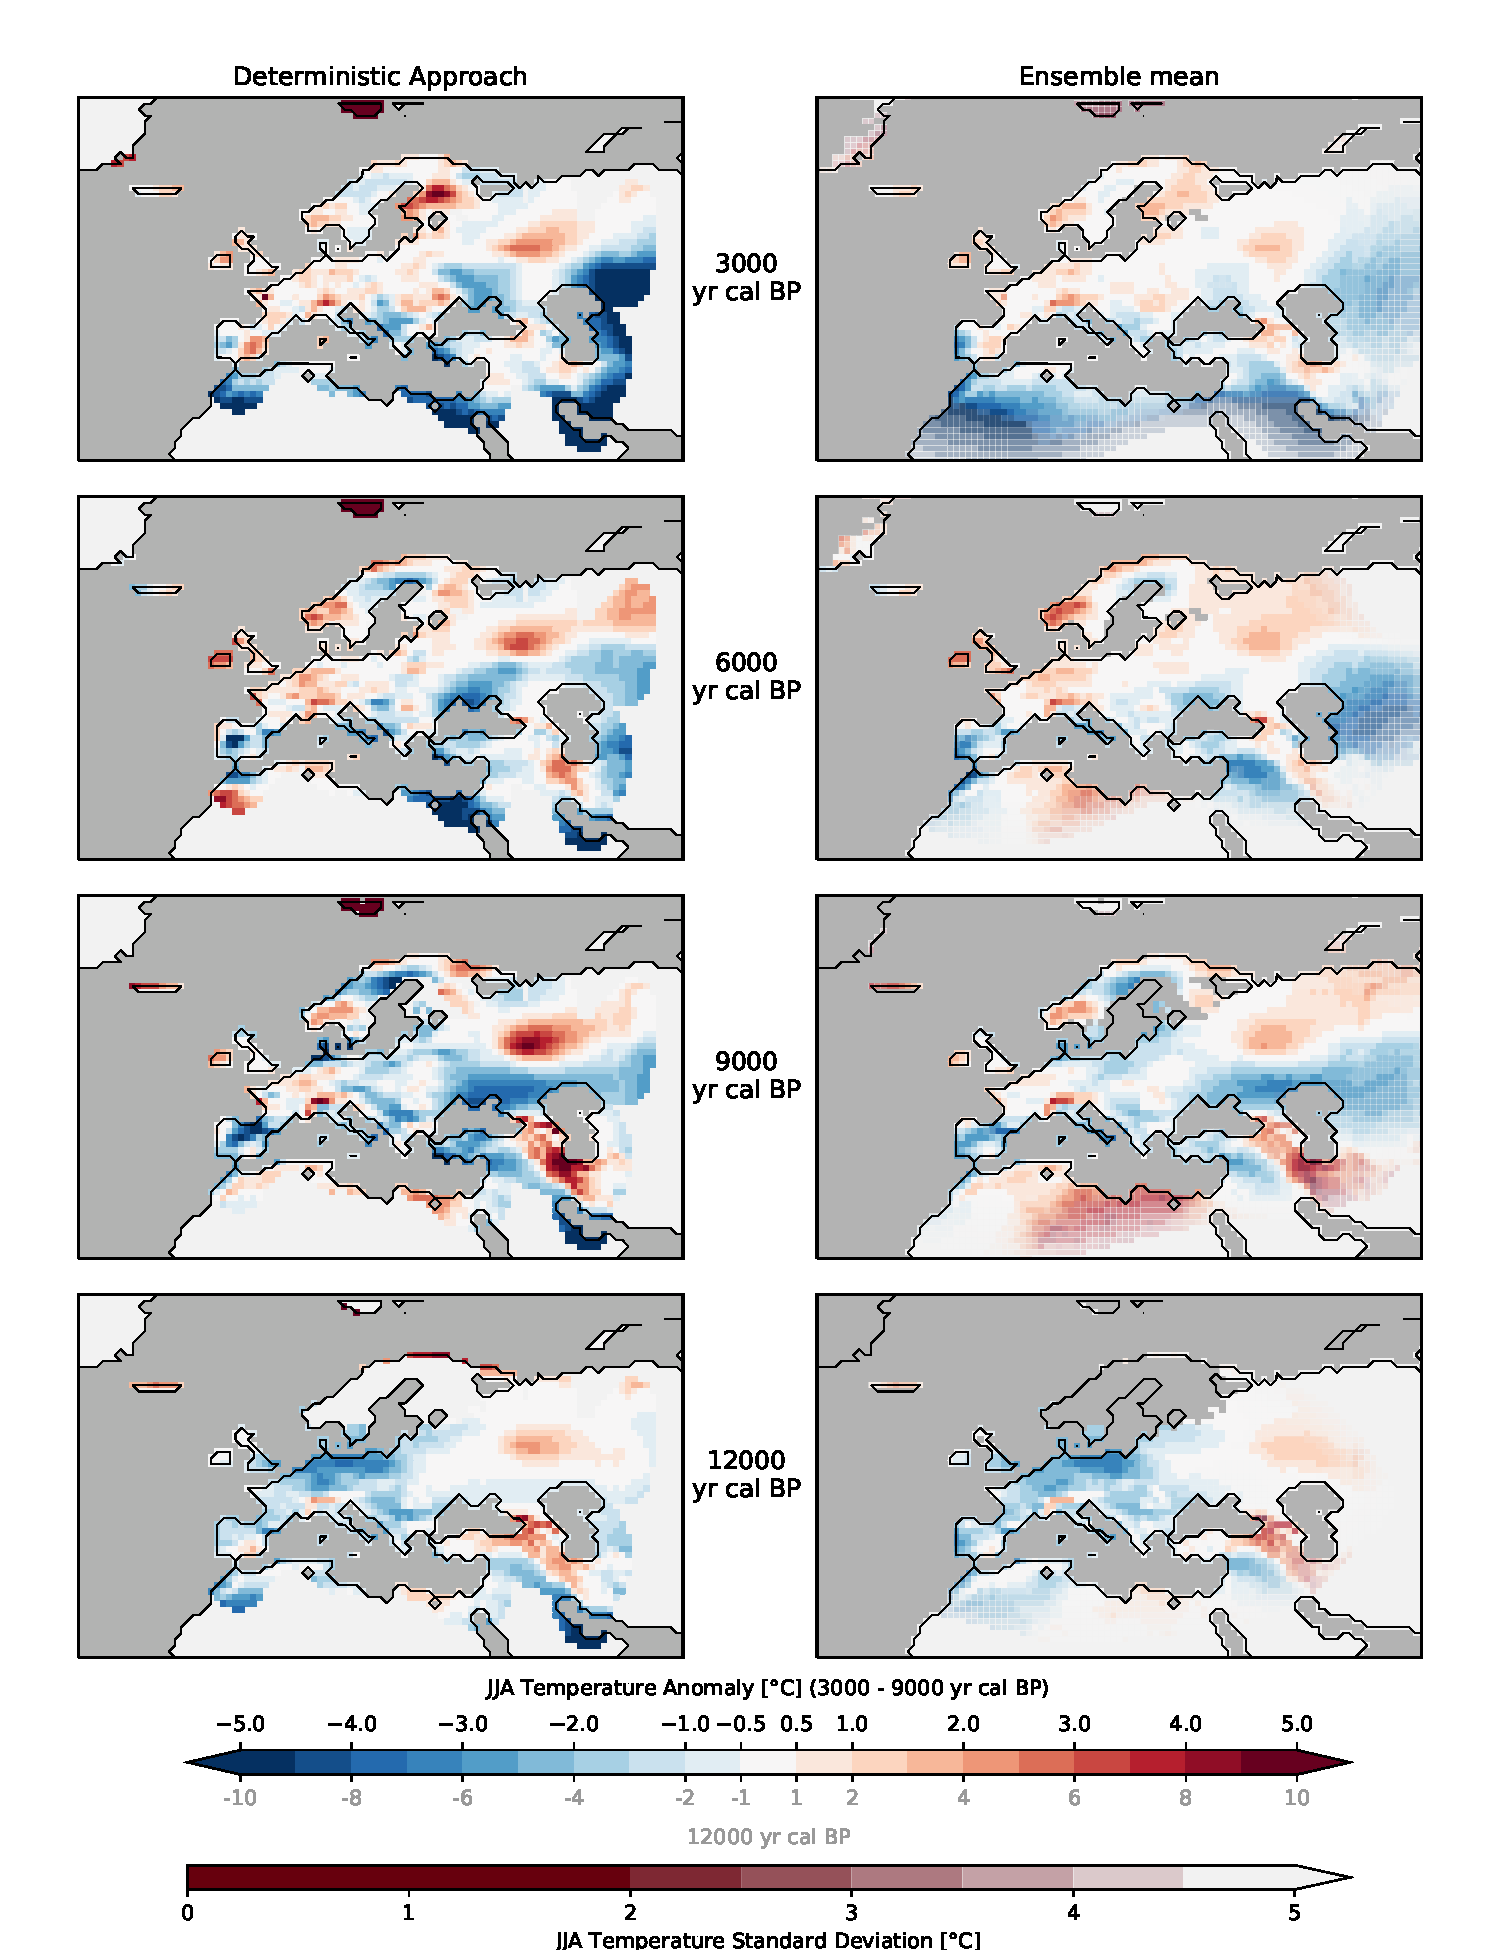
\includegraphics[width=\linewidth]{gridding-figures/deterministic-vs-ensemble.pdf}
	\caption[Deterministic approach vs. Ensemble mean]{Deterministic approach vs. ensemble mean (10'000 realizations) at 3k, 6k, 9k and 12k BP (note the different color coding for 12k BP). Each map shows the anomaly with respect to the gridded reconstruction at 0k BP. The deterministic approach (left column) is the input data with temperatures as weighted averages of the 50 closest analogues and without age sampling. The gridded reconstruction has been masked when more than 500km away from the closest sample. The ensemble mean (right column) is overlayed by the corresponding ensemble standard deviation of the anomaly (suppl. figure \ref{fig:gridding-gridded-std}). This overlay is transparent for standard deviations smaller than 2.5 °C and afterwards gets more opaque until it reaches 5 °C. Grid cells in the maps that were covered by more than 50 percent with ice, according to the ICE-6G data, have been masked.}
	\label{fig:gridding-gridded-mean}
\end{figure}

The gridded reconstruction for the entire dataset is shown in figure \ref{fig:gridding-gridded-mean} for 3k, 6k, 9k and 12k BP. The figure shows the temperature anomaly to the modern time (0k BP), both for the ensemble method (10'000 realizations, 5 °C climate constraint) and the deterministic case, i.e. without climate and temperature sampling. For the deterministic case, we followed the approach by \cite{MauriDavisCollinsEtAl2015} and mask cells that are further away than 500km from any of the pollen sites. For the ensemble approach on the other hand we used the ensemble standard deviation as a gray overlay that is getting more opaque for higher standard deviations.

Both methods show similar patterns and span the same temperature range at the onset of the Holocene. The temperature ranges in the other maps, however, are different with the deterministic approach being more extreme in certain locations, particularly in Spain, eastern Russia and the western Mediterranean region. The method predicts absolute temperature anomalies of more than four degrees, whereas the anomalies of the ensemble approach commonly range between -2.5 and 2.5 °C are more coherent. The ensemble standard deviation of the anomaly (suppl. figure \ref{fig:gridding-gridded-std}) in Europe ranges between 0.5 and 1 °C for the mid- to late Holocene timesteps at 6k and 3k BP, and between 1 and 2 °C at 12k and 9k BP. The standard deviation is particularly high at the map boundaries of the 12k reconstruction, very likely due to the smaller availability of fossil samples in this period.


\subsubsection{Temperature sampling parameters}

\begin{figure}
	\includegraphics[width=\linewidth,page=3]{gridding-figures/temperature-means-per-thresh.pdf}
	\caption[Impact of climate constraint on gridded results]{Ensemble mean summer temperature anomaly at 9k BP (1'000 realizations) for different temperature constraints. The standard deviation is visualized on top of the mean with an increasing opaqueness (same as in figure \ref{fig:gridding-gridded-mean}).}
	\label{fig:gridding-gridded-climate-constraint}
\end{figure}

\begin{figure}
	\includegraphics[width=\linewidth,page=3]{gridding-figures/temperature-means-per-k.pdf}
	\caption[Impact of the number of analogues on the gridded results]{Ensemble mean summer temperature anomaly at 9k BP for numbers of analogues. The standard deviation is visualized on top of the mean with an increasing opaqueness (same as in figure \ref{fig:gridding-gridded-mean}).}
	\label{fig:gridding-gridded-k}
\end{figure}

Figure \ref{fig:gridding-gridded-climate-constraint} shows the influence of the choice for the climatic constraint (see section \ref{sec:gridding-temperature-sampling}) on the gridded reconstruction for a selected timestep at 9k BP. The comparison of the 5 °C and the very relaxed 10 °C constraint shows only minor differences. Stronger constraints (2 °C and 3 °C) result in a strengthening of the anomaly, particularly in Spain and towards the southern and south-eastern borders of the map. These impacts are coherent with a reduced number of analogues, as shown in figure \ref{fig:gridding-gridded-k}. Lower numbers of analogues, e.g. 6 or 10, result in a similar strengthening of the anomaly in these geographic regions.


\subsubsection{Uncertainties for spatial extrapolation}

\begin{figure}
	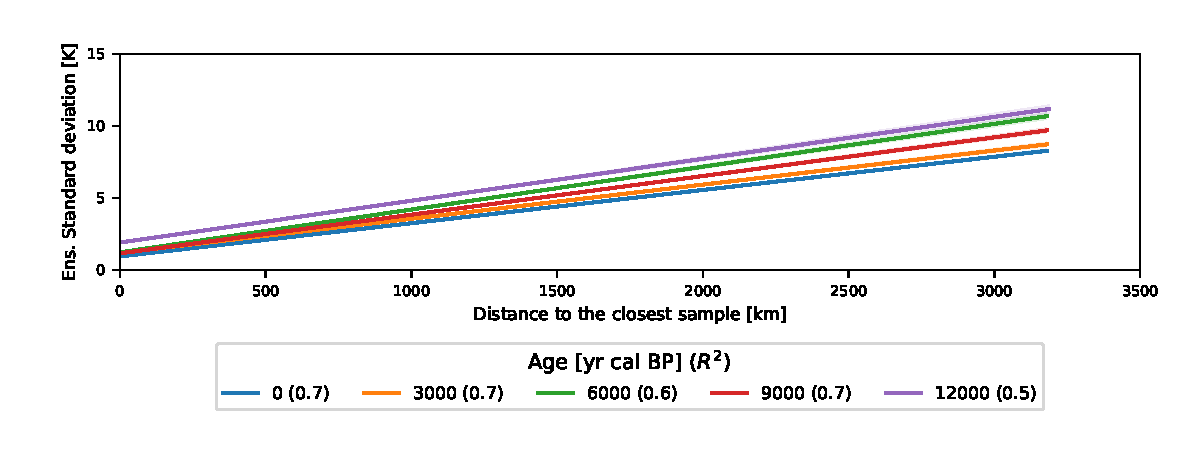
\includegraphics[width=\linewidth]{gridding-figures/distance-std-relation.pdf}
	\caption[Relationship between distance to proxy sites and ensemble standard deviation]{Relationship between distance to proxy sites and the ensemble standard deviation. Each line corresponds to a linear fit where the distance to the closest site in the database for a given grid cell is regressed against the ensemble standard deviation in this cell (figure \ref{fig:gridding-gridded-std}). The different lines represent the different time steps from figure \ref{fig:gridding-gridded-mean}, the value in brackets after each legend label shows the coefficient of determination ($R^2$) for the given regression fit.}
	\label{fig:gridding-dist-std}
\end{figure}

One important issue of gridding is the question about how far we can extrapolate spatially outside of the geographic domain of our proxy database. \cite{MauriDavisCollinsEtAl2015} for instance chose a fixed threshold of 500km to the closest pollen site (also shown in the deterministic plots of figure \ref{fig:gridding-gridded-mean}). Grid cells that are further away than this, are masked.

The ensemble method we present here does not require such a formal definition and should rather be interpreted with respect to the calculated uncertainties. Figure \ref{fig:gridding-dist-std} shows a clear linear relationship between this distance and the ensemble uncertainty. It also reveals the caveats of using fixed threshold because the relationship between standard deviation and distance to the closest site is time dependent, likely because of the smaller amount of available samples during the early Holocene.

\section{Discussion}  \label{sec:gridding-discussion}
In this section, we will discuss the methodological uncertainties of the method that are not necessarily easy to quantify. They arise from first, the underlying site-based proxy-climate reconstruction method (in this case \gls{mat}), second the constrained climate sampling to approximate the joint distribution, and third, the gridding algorithm (\textit{Tps}).

The results from the side-based reconstruction in section \ref{sec:gridding-site}, and the gridded reconstruction in section \ref{sec:gridding-gridded-results}, show that the first two aspects (site-based reconstruction method uncertainty and climate sampling) are closely linked, and potentially have a strong influence on the outcome. The effects of a reduced number of analogues (figures \ref{fig:gridding-tigal-recon-k} and \ref{fig:gridding-gridded-k}), as well as a stronger climatic constraint (figures \ref{fig:gridding-tigal-recon} and \ref{fig:gridding-gridded-climate-constraint}) resulted in more extreme temperature anomalies over the same geographic regions. This result is coherent with the sampled temperatures presented in the methods section (figure \ref{fig:gridding-temp-sampling-violins}) where we show that a higher climatic constraint particularly strengthens the closer climate analogues and as such effectively reduces the number of  analogues that is used in the reconstruction. There is no clear and definitive answer to the question how many analogues one should use and how strong the climatic constraint should be. Based on the results however, we favor a less strong climatic constraint of 5 °C and a high number of analogues (50). The philosophy behind is to let the method choose which analogue it uses. If there are inconsistencies within the set of modern analogues for a particular dataset, then this should be reflected by the ensemble standard deviation, and can eventually be compensated by the spatially neighboring samples in the gridding process.

These are all problems that arise from the underlying discrete distribution of modern analogues. An alternativity would be to use a PDF based method \citep[for instance]{ChevalierCheddadiChase2014, Chevalier2019} that can potentially overcome these weeknesses by providing a more continuous distribution for sampling the climate.

The third aspect of the uncertainty is related to the gridding algorithm itself which can be added on top of the uncertainty of our ensemble method. For the \textit{Tps} method, this uncertainty can be estimated conveniently using the \textit{predictSE} function of the \textit{fields} R-package that approximates the covariances of the prediction based on a linear combination of the observed data under the assumption of fixed covariance parameters (see \cite{NychkaFurrerPaigeEtAl2017} for details). A calculation of this standard error for 20 ensemble members revealed that it is rather independent of the individual realization. As such, we present the averaged standard error of these 20 members in the supplementary figure \ref{fig:gridding-tps-se}. We can see that this uncertainty estimate is high towards boundaries of the interpolation domain, but smaller than the ensemble standard deviations in between.


\section{Conclusions}  \label{sec:gridding-conclusions}
With \textit{pyleogrid} we are presenting a new methodological framework that transforms multiple site-based proxy-climate reconstructions into a joint spatio-temporal probabilistic climate reconstruction. Our method exploits the climatic and temporal space that is spanned by the intrinsic uncertainties related to the proxy-climate reconstruction method and the dating of the samples, in order to approximate the distribution of potential climate states in the geographic area of interest. Our approach requires little parametrization, is computationally efficient and can be scaled to large hemispheric or even global areas. The generic ensemble approach we present is in principle agnostic to the underlying proxy-climate reconstruction method and to the gridding method and can therefore be extended to a wide range of potential applications.

Compared to previous approaches of a large-scale gridded reconstruction, our method therefore provides a more reliable uncertainty estimate based on our constrained sampling approaches, which is essential for the comparison with climate model output. 

The methodology comes with two side-products that are essential for the spatio-temporal ensemble approach. The first one is a methodology to estimate dating uncertainties based on a bivariate model of the age of the sample and its temporal distance to the closest chronological control point in the dataset. The other side-product, is a probabilistic variant of the site-based \glsfirst{mat} that uses a Gibbs sampling algorithm for the ages and analogue climates in order to approximate the joint distribution within a single dataset. This sampling algorithm is constrained for the individual dataset through first, the monotonicity of the sample ages, and second, a climatic threshold that must not be overcome between too temporally neighboring samples. We compare this sampling algorithm to computationally faster algorithms that involve a forward sampling (climate/age of a sample is constrained by it's younger predecessor), its inversion, the backward sampling, as well as a combined approach that uses forward and backward sampling. For age sampling we also test an algorithm that starts with an unconstrained sampling of the ages and then applies an a posteriori sorting in order to maintain the correct distribution of samples in the core (sections \ref{sec:gridding-age-sampling} and \ref{sec:gridding-temperature-sampling}). All of these approaches, however reveal biases when compared to the computationally more demanding, but stationary correct distribution of the Gibbs sampler. The software package \textit{pyleogrid} therefore implements a computationally efficient version of this Gibbs sampling algorithm that efficiently scales from one single dataset to tenth of thousands of realizations of more than a thousand individual datasets, as it has been used in this study.

This sampling successfully reconstructs a probabilistic version of the individual dataset and provides reliable uncertainty estimates. An evaluation of this realization with respect to the number of modern analogues, and the climatic constraint of the sampling algorithm reveals a close linkage of the two parameters. Further developments might therefore explore the usage of other proxy-climate reconstruction methods that provide a more continuous distribution to sample from.

\clearpage

\begin{subappendices}
	\section*{Supplementary material}
	
	\section{Estimated age uncertainties}  \label{sec:gridding-suppl-age-uncertainties}	
		\begin{figure}[!h]
			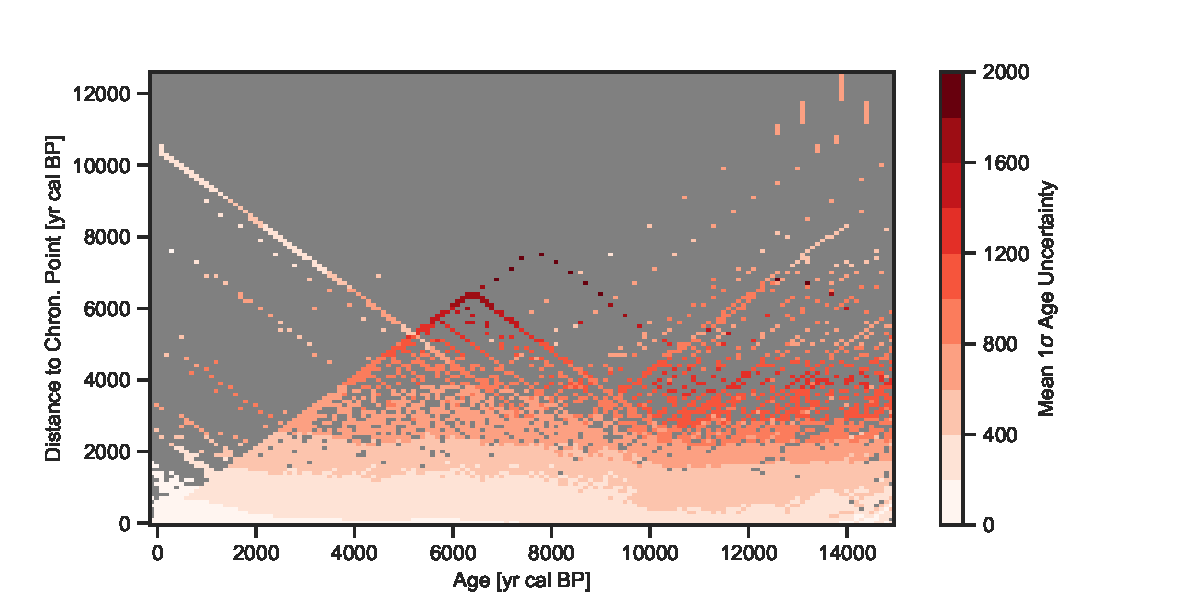
\includegraphics[width=\linewidth]{gridding-figures/realized-age-uncertainties.pdf}
			\caption[Estimated age uncertainties]{Estimated age uncertainties for the Eurasian dataset from section \ref{sec:gridding-polnet} with the same formatting as in figure \ref{fig:gridding-bivariate-age-unc}.}
			\label{fig:gridding-age-uncertainties}
		\end{figure}

	\section{Example of generated age distributions} \label{sec:gridding-suppl-age-example-distributions}
		\begin{figure}[!h]
			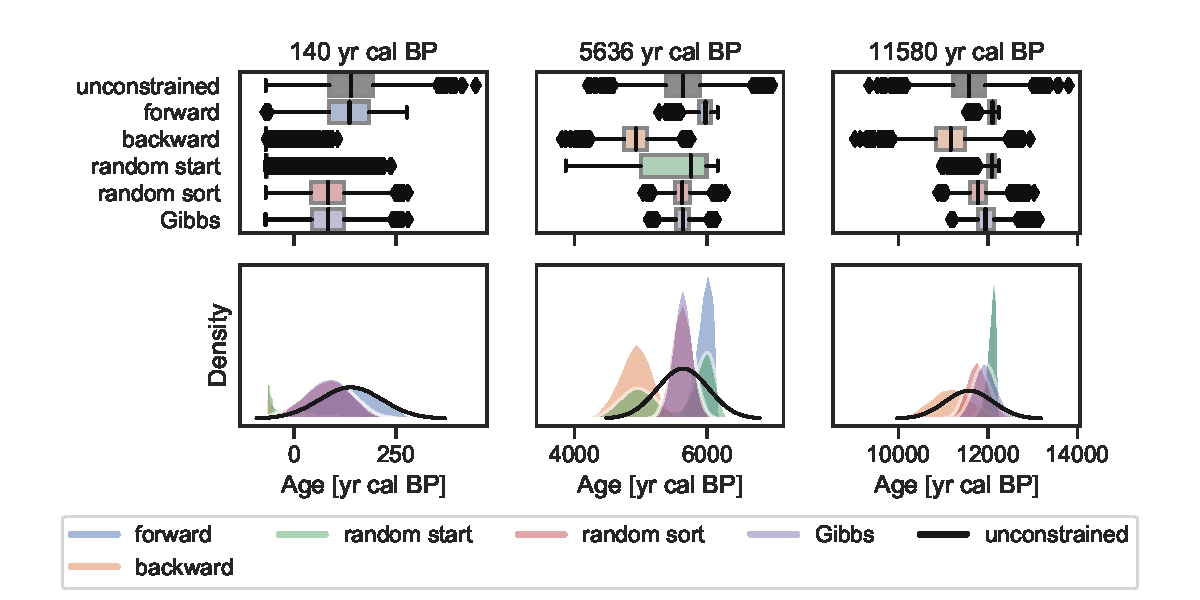
\includegraphics[width=\linewidth]{gridding-figures/age-sampling-methods-use-case.pdf}
			\caption[Example of sampled distribution]{Example of three samples from the site in section \ref{sec:gridding-site} and their realized distributions. Sampling algorithms are explained in section \ref{sec:gridding-age-sampling}. Top plots show the box plots of the realized distribution that are visualized with a kernel density estimate in the lower row.}
			\label{fig:gridding-age-example-distributions}
		\end{figure}
	
	\section{Maps of uncertainties} \label{sec:gridding-suppl-maps}
		\begin{figure}[h]
			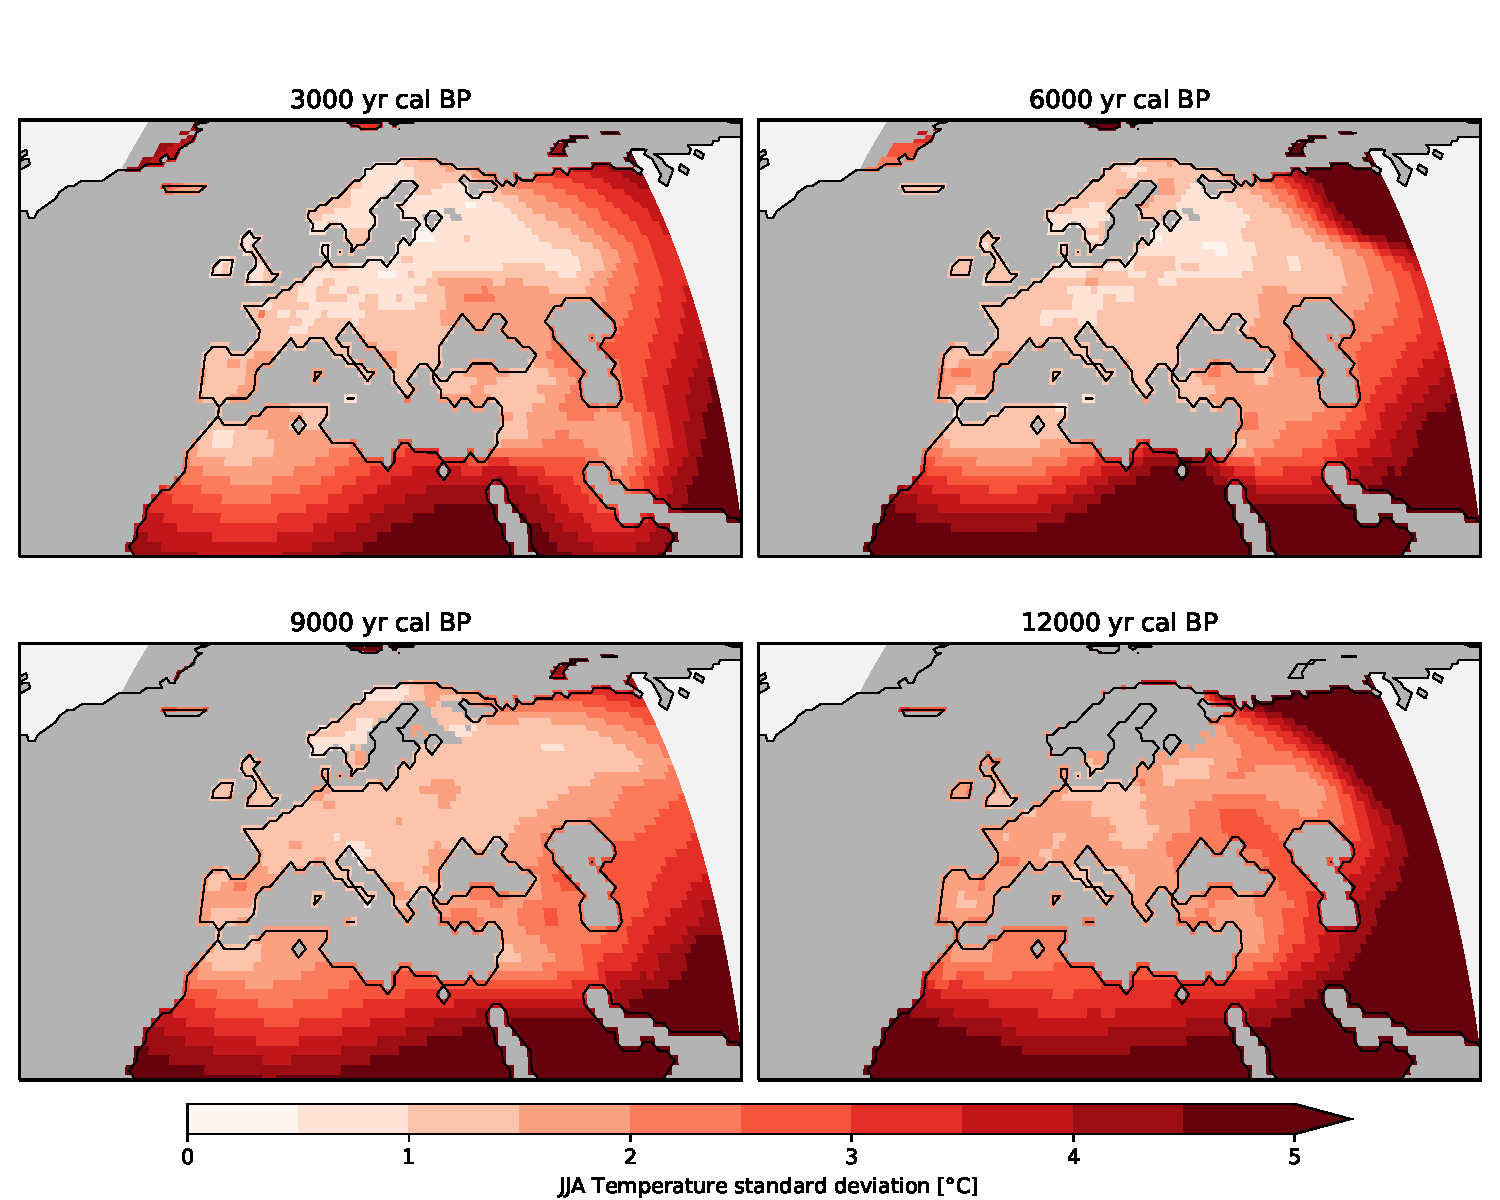
\includegraphics[width=\linewidth]{gridding-figures/ensemble-std.pdf}
			\caption[Ensemble standard deviation]{Standard deviation of the ensemble mean summer temperature anomaly (10'000 realizations) at 3k, 6k, 9k and 12k BP.}
			\label{fig:gridding-gridded-std}
		\end{figure}
	
		\begin{figure}[h]
			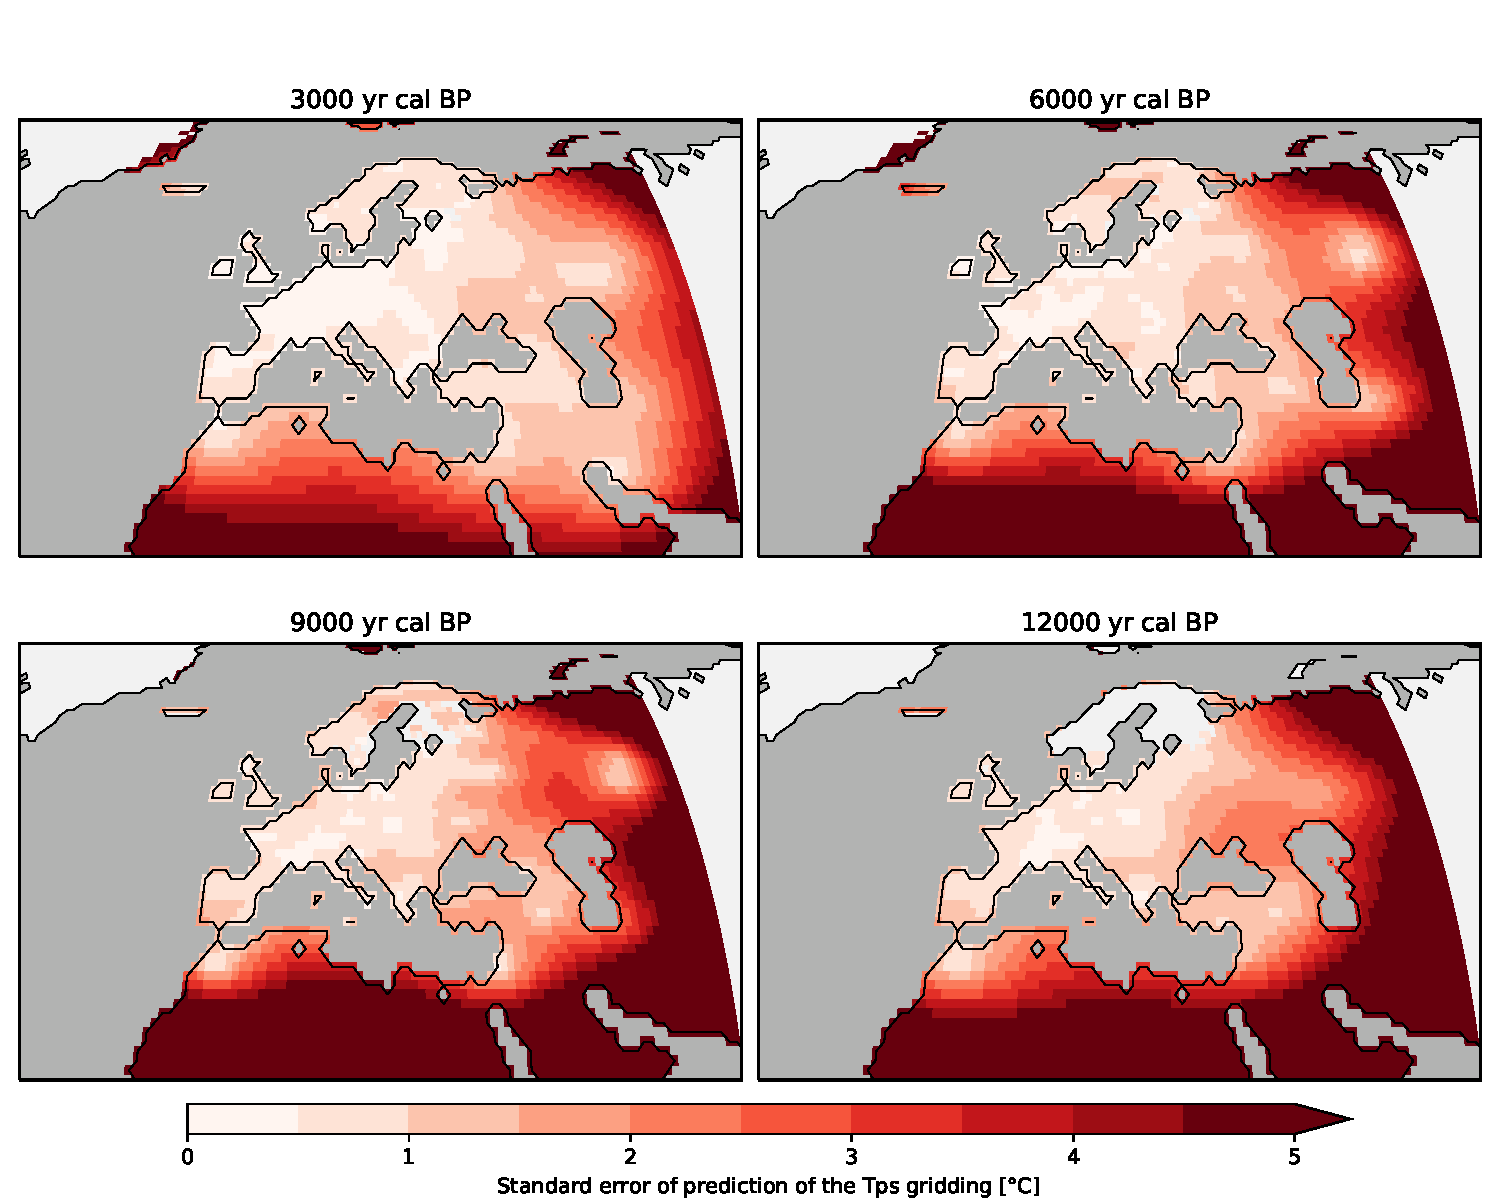
\includegraphics[width=\linewidth]{gridding-figures/ensemble-tps-se.pdf}
			\caption[Standard error of the Tps gridding method]{Standard error of the gridding algorithm, predicted with the \textit{predictSE} method of the \textit{fields} package \citep{NychkaFurrerPaigeEtAl2017} for the different timeslices. The standard errors are an average of 20 ensemble members, although there is only very little difference between the individual maps.}
			\label{fig:gridding-tps-se}
		\end{figure}

\end{subappendices}

\clearpage

\printbibliography[heading=subbibintoc]

\end{refsection}